\documentclass[a4paper]{amsart}
\usepackage{amssymb,amsmath,amsthm,amsfonts}
\usepackage{epsfig}
\usepackage{color}
\usepackage{subfloat}
\usepackage{verbatim} % block comments
\usepackage{import} % figures in a separate directory
\usepackage{url} % urls

\newtheorem{thm}{Theorem}[section]
\theoremstyle{remark}
\newtheorem{rem}[thm]{Remark}

% sixth iterate of poincare map, P^{6}
\newcommand{\sixmap}{\mathcal{P}}

\newcommand{\field}[1]{\mathbb{#1}}
\newcommand{\RR}{\mathbb{R}}


\begin{document}
\title{Numerical measure of splitting angle}
\author{J.~F\'ejoz, V.~Kaloshin, M.~Guardia, P. Rold\'an}

\begin{abstract}
Goal: measure splitting of stable/unstable manifolds of a resonant periodic
orbit in the Sun-Jupiter RTBP.
\end{abstract}
\maketitle

\section{Periodic Orbit} \label{sec:periodic_orbit}

\subsection{2-body problem}

Vadim has provided us an initial condition that corresponds to a 7:1 resonant
periodic orbit in Kepler's problem (polar coordinates)
\[ H=\frac{1}{2}(R^2+\frac{\Theta^2}{r^2})-\frac{1}{r}. \]
The initial condition is at the perihelion,
\[(r,R,\theta,\Theta)=(1.302533194, 0.0, 0.0, 1.46336205),\]
or equivalently in euclidean coordinates
\[(x,y,v_x,v_y)=(1.302533194, 0.0, 0.0, 1.123473908).\]
This periodic orbit lives in the energy level $H=-1.6$.

In fact, we have a program that, given an energy value $H$, computes an initial
condition of Asteroid $(x,y,v_x,v_y)$ corresponding to $r=p/q$ ressonant
periodic orbit in the 2BP. 
Here, $p$ is period of asteroid and $q$ is period of Jupiter.
We impose that initial condition is at the perihelion. This implies that
position of Asteroid is $A=(x,0)$ and velocity is $v=(0,v_y)$.
Therefore, we output as initial condition only the components
$(x,v_y)$.

\begin{verbatim}
roldan@pollo:~/research/splitting/initcond$ initcond 
-1.6 7                                        # input: H r=p/q
1.302533194285694e+00 1.123473908222282e+00   # output: x v_y
\end{verbatim}

First of all, we check that this initial condition is correct. An analytical
integration of Kepler's equations gives the particular solution
\[ u=1/r, \quad u(\theta)=1/c^2(1+\epsilon \cos(\theta-g)), \]
with constant angular momentum $c=1.46336205$, eccentricity $\epsilon =
0.644049091$, and argument of the perihelium $g=0$.
Since $0<\epsilon<1$, it is an ellipse.

Moreover, we have integrated the trajectory numerically, and indeed we obtain
a periodic orbit of period $T=14\pi$ with high precision. Program "ikepler"
integrates the trajectory:

\begin{verbatim}
roldan@pollo:~/research/splitting/ikepler$ ./ikepler <ikepler.dat
0.000000e+00 1.302533e+00 0.000000e+00 0.000000e+00 1.463362e+00
...
4.398230e+01 1.302533e+00 -2.501898e-08 6.283185e+00 1.463362e+00
\end{verbatim}
The first line corresponds to the initial condition $(t=0,r,R,\theta,\Theta)$
and the last line to the final point $(t=14\pi,r,R,\theta,\Theta)$. Note that
they only differ by $10^{-8}$ (the first column is just time, and the fourth
column is an angle, so $6.283185e+00=0$ $(\mod 2\pi)$.

\begin{figure}[!htbp]
\subincludefrom{figs/}{ikepler}
\caption{Integration of Kepler's problem: analytical trajectory in red,
numerical in green.}
\label{fig:ikepler}
\end{figure}

See a plot of the trajectory in figure~\ref{fig:ikepler}.

\subsection{3-body problem}

Now we switch to the (circular, planar) RTBP equations (in synodical, or
rotating, coordinates)
\begin{equation}\label{eq:RTBP}
H(x,y,p_x,p_y)=
\frac{1}{2}(p_x^2+p_y^2)+yp_x-xp_y-\frac{\mu_1}{r_1}-\frac{\mu_2}{r_2},
\end{equation}
where 
\begin{align*}
r_1^2 &= (x-\mu_2)^2 + y^2, \\
r_2^2 &= (x+\mu_1)^2 + y^2.
\end{align*}

We follow the convention to place the large mass (Sun) to the left of
the origin, and the small mass (Jupiter) to the right.
(This is opposite to the astrodynamics convention).
Thus we choose $\mu_1=\mu$ as the small mass, and $\mu_2=1-\mu$ as the
large mass.

We would like to check that the initial condition for the 2BP is still a good
approximation to a resonant periodic orbit in the RTBP. 

As a first test, we consider the RTBP~\eqref{eq:RTBP} with $\mu=0$. This is
just the 2BP in rotating coordinates (position-momentum instead of
position-velocity). We need to express the initial condition in these RTBP
coordinates. Note that the origin is still located at the Sun. Since the
initial condition is at the perihelion, at $t=0$ the rotating and fixed frame
coincide, so ${(x,y)}_{\mathrm{2BP}}={(x,y)}_{\mathrm{RTBP}}$. 

Moreover, remember the interpretation of momenta in the rotating system:
$p_x,p_y$ are the components of the velocity (wrt the fixed system) along the
rotating axes (see Szebehelly, page 349). Again, since the rotating and fixed
frame coincide, 
${(v_x,v_y)}_{\mathrm{2BP}}={(p_x,p_y)}_{\mathrm{RTBP}}$.
Thus, it turns out that
\[ {(x,y,p_x,p_y)}_{\mathrm{RTBP}} = {(x,y,v_x,v_y)}_{\mathrm{2BP}} =
(1.302533194, 0.0, 0.0, 1.123473908). \]

Again, we compare the initial and final points after integrating time
$14\pi$. Program "frtbp" computes the flow of the RTBP. 

\begin{rem}
We use a variable-order taylor method specially generated to integrate
the equations of motion of the RTBP. 
The taylor method has been generated using the "taylor" package of \`{A}.~Jorba
and M.~Zou (see~\url{http://www.maia.ub.es/~angel/taylor/}).
The main advantage of using a taylor method is that it is very fast
for long-time integrations (without sacrificing accuracy).
\end{rem}

\begin{verbatim}
roldan@pollo:~/research/splitting/frtbp$ frtbp 
0                                                     # input: mu
43.98229715025710533816                               # input: 14\pi
1.302533194285694e+00 0.0 0.0 1.123473908222282e+00

# output:
1.302533194285696e+00 -3.183137881087434e-13          # x, y
1.708491712633289e-13 1.123473908222281e+00           # p_x, p_y
\end{verbatim}
We input mass parameter $\mu=0$ (first line), integration time $t=14\pi$
(second line), and initial condition (third line). The program outputs the
final point (fourth line). Notice that the distance between initial and final
point is about $10^{-13}$. Therefore we obtain a resonant periodic orbit.

As a second test, we consider the RTBP~\eqref{eq:RTBP} with
$\mu=0.95387536e-3$, the mass ratio of Sun-Jupiter. Of course, the Sun is not
located at the origin anymore, but nevertheless we hope that the same initial
condition
\[ {(x,y,p_x,p_y)}_{\mathrm{RTBP}} = (1.302533194, 0.0, 0.0, 1.123473908) \]
gives rise to a trajectory that is close to a resonant periodic orbit. Let's
check it again by applying the flow time $14\pi$:

\begin{verbatim}
roldan@pollo:~/research/splitting/frtbp$ frtbp 
0.95387536e-3
43.98229715025710533816
1.302533194285694e+00 0.0 0.0 1.123473908222282e+00

# output:
1.250163242561269e+00 -4.990618523763478e-01 
2.444851824792766e-01 1.076199186094388e+00
\end{verbatim}
and we see that the final and initial points (third and fourth lines) differ
by about $10^{-1}$. Therefore we are close to a resonant periodic orbit of
the RTBP.

Next we refine the approximate periodic orbit into a "true" periodic orbit
(up to numerical integration errors).
Consider the Poincare section 
\[ \Sigma = \{ y=0,\ p_y>0 \} \] 
in the autonomous RTBP~\eqref{eq:RTBP}, and let $P\colon\
\Sigma\to\Sigma$ be the associated Poincare map.

Notice that, in the rotating frame, a 7:1 resonant periodic orbit
makes $6$ turns around the origin.
We look for the periodic orbit as a fixed point of the map
\[ \sixmap \equiv P^6, \] 
which is the $6$-th iterate of the Poincare map.
We will refer to $\sixmap$ as the \emph{iterated Poincare map}.

\begin{rem}
Due to some symmetry of the RTBP equations w.r.t. the horizontal axis,
in fact it is only necessary to integrate for half a period of the
periodic orbit. We will exploit this fact in
section~\ref{sec:symmetric_periodic_orbits}.
\end{rem}

For instance, let us compute the image $p'=\sixmap(p)=P^6(p)$ of the point
$p=(x,y,p_x,p_y)=(1.302533194,0.0,0.0,1.123473908)$, which corresponds
to our guess to the periodic orbit. 
Of course, we expect this to be close to a fixed point.

\begin{rem}
Numerical remark: 
A point is assumed to be on the Poincare section if it is within distance
$10^{-16}$ to the section.
\end{rem}

\begin{verbatim}
roldan@pollo:~/research/splitting/prtbp$ ./prtbp
0.95387536e-3                           #input: mu
6                                       #input: number of iterates
#input: (x,y,p_x,p_y)
1.302533194285694e+00 0.0 0.0 1.123473908222282e+00
#output:
1.693695656893852e+00                   # x'
4.879248589363672e-16                   # y'
-4.007796441169778e-01                  # p_x'
8.653917332089469e-01                   # p_y'
4.285874020770370e+01                   # integration time
\end{verbatim}
Thus the Poincare iterate is very close to the input point.
Moreover, as a side product, we also compute the integration time needed to
reach the Poincare section. This number is of course close to
$14\pi=43.982\dots$.

To further reduce dimensionality, fix the level of energy to
\begin{equation}\label{eq:energy}
H(x,y,p_x,p_y)=H_0=-1.6
\end{equation}
We look for the periodic orbit \emph{in the energy manifold} $H_0$.

*** Does there exist a periodic orbit for every value of the energy
close to $H_o$??? I guess so. ***

*** If there exists one, is it exactly resonant (i.e. does it have the
\emph{exact} period $14\pi$)??? I guess not. Maybe we can look for the exact
resonant periodic orbit by varying the energy level.
***

Using this energy condition~\eqref{eq:energy}, we can work with only two
variables, $(x,p_x)$.
The variable $y=0$ since we look at the Poincare section. Further, suppose
$\partial H/\partial p_y \neq 0$ so we can apply IFT, and the variable $p_y$
can be obtained from the energy condition~\eqref{eq:energy}. 
Given $x,p_x,y$ and $H$, we just need to solve a quadratic equation for
$p_y$.

\begin{verbatim}
roldan@pollo:~/research/splitting/hinv$ ./hinv 
0.95387536e-3 -1.6                                   #input: mu, H
1.302533194285694e+00 0.0 0.0 1.123473908222282e+00  #input: p
hinv: I have chosen branch number 2
1.113427091316086e+00                                #output: p_y
\end{verbatim}

For instance, let us compute the 2-dimensional Poincare map
$\sixmap(p)$ of the point $p=(x,p_x)=(1.302533194,0.0)$, which
corresponds to our guess to the periodic orbit. 
Of course, we expect this to be close to a fixed point.

\begin{verbatim}
roldan@pollo:~/research/splitting/prtbp$ ./prtbp_2d
0.95387536e-3                           #input: mu 
-1.6                                    #input: H
6                                       #input: number of iterates of P
1.302533194285694e+00 0.0               #input: (x,p_x) 
1.123473908222282e+00                   #input: p_y estimate

#output: (x',p_x') integration_time
hinv: I have chosen branch number 2
3.664378990446215e+00 3.061299749188896e-01 4.633168561934585e+01
\end{verbatim}
Notice that we do not obtain the same point as with the 4D Poincare
map. This is due to the fact that we are using an energy level
$H=-1.6$ which, \emph{for the RTBP}, does not correspond to the point
$(x,y,p_x,p_y) = (1.3025, 0, 0, 1.1234)$. This was true only in the 2BP.

The corresponding energy level for the RTBP is 
\[ H(x,y,p_x,p_y) = -1.60184944512740670488. \]
 Let us now use this energy level.

\begin{verbatim}
roldan@pollo:~/research/splitting/prtbp$ ./prtbp_2d
0.95387536e-3
-1.60184944512740670488 
6
1.302533194285694e+00 0.0
1.123473908222282e+00

#output: (x',p_x') integration_time
hinv: I have chosen branch number 2
1.693695656894214e+00 -4.007796441170626e-01 4.285874020770324e+01
\end{verbatim}
Of course, now we obtain the same point as with the 4D Poincare map.

Next we compute the derivative of the Poincare map.
For each $\xi\in R^4$, let $u(t,\xi)$ be the solution of the system with
initial condition $u(0,\xi)=\xi$. 
Let $\Sigma$ be the Poincare section $\{y=0\}$, and $T:\Sigma\to R$ the
Poincare return time. 
The derivative of the Poincare map at a point $p$ is given by the partial
derivative $u_\xi(T(p),p)$.
It is easy to see that $u_\xi(t,p)$ is the matrix solution of the variational
equation
\[ \dot W = Df(u(t,p))W, \]
where $f$ is the vectorfield of the RTBP.
We compute $u_\xi(T(p),p)$ by numerically integrating the variational
equations.

\begin{verbatim}
roldan@pollo:~/research/splitting/dprtbp$ ./dprtbp
0.95387536e-3                         #input: mu 
6                                     #input: number of iterates 
#input: p=(x, y, p_x, p_y)
1.302533194285694e+00 0.0 0.0 1.123473908222282e+00

#output: u_\xi(T(p),p)
 1.163429283356999e+02 -5.605786501223135e+00 -2.674694568710321e+00  2.199226681825827e+02
-2.477782902512909e+02  1.000758275840821e+01  1.835082184567418e+00 -4.727484205470752e+02
 9.942019451626798e+01 -3.778309795557094e+00 -3.066006635286664e-01  1.891231152838540e+02
 5.840932484939698e-03  4.749823112392679e-01  9.251703062627508e-01  5.696378415895288e-01
\end{verbatim}

Next we compute the derivative of the 2D Poincare map.
Let $H(x,y,p_x,p_y)$ be the Hamiltonian of the RTBP~\eqref{eq:RTBP}.
Let $f=(f_1,...,f_4)$ be the vectorfield of the RTBP.
Let $u(t,\xi)=\phi_t(\xi)$ be the flow of the RTBP.
Let 
\[ u_\xi(T(p),p)=(u_{ij})_{i,j=1,\dots,4}\] 
be the variationals, i.e. the derivative of the 4D Poincare map.

We want to compute
\[ DP(x,p_x) = 
\begin{pmatrix}
D_{11} & D_{12} \\
D_{21} & D_{22}
\end{pmatrix}.
\]
Let us compute $D_{11}$ for example. Consider the first component of the 2D
Poincare map, $P_1(x,p_x) = u_1(T(p),p) = u_1(T,x,0,p_x,p_y(x,p_x))$. Take
the partial derivative
\[ D_{11} = \frac{\partial P_1}{\partial x} = 
\frac{\partial u_1}{\partial x} + 
\frac{\partial u_1}{\partial p_y} \frac{\partial p_y}{\partial x} +
\frac{\partial u_1}{\partial T} \frac{\partial T}{\partial x}.
\]
The following data is known:
\[
\frac{\partial u_1}{\partial x} = u_{11}, \quad
\frac{\partial u_1}{\partial p_y} = u_{14}, \quad
\frac{\partial u_1}{\partial T} = f_1(u(T,p)).
\]
It remains to find $\frac{\partial p_y}{\partial x}, \frac{\partial
T}{\partial x}$. Consider the energy condition
\[ H(x,0,p_x,p_y(x,p_x)) = h. \]
Derivating wrt $x$, we obtain:
\[ \frac{\partial p_y}{\partial x} = 
-\frac{\partial H/\partial x}{\partial H/\partial p_y} = 
\frac{f_3(p)}{f_2(p)}. \]
Consider the Poincare section condition
\[ u_2(T,x,0,p_x,p_y(x,p_x)) = 0. \]
Derivating wrt $x$, we obtain:
\[ \frac{\partial T}{\partial x} = -\frac{1}{f_2(u(T,p))} 
\left( u_{21} + u_{24} \frac{\partial p_y}{\partial x} \right).
\]
Therefore 
\[ D_{11} =
u_{11} + u_{14} \frac{f_3}{f_2} + f_1(u(T,p)) 
\left( -\frac{1}{f_2(u(T,p))}\left( u_{21} + u_{24} \frac{f_3}{f_2} \right) \right).
\]
Similarly, we have
\begin{align*} 
D_{12} &= u_{13} - u_{14} \frac{f_1}{f_2} + f_1(u(T,p))
\left( -\frac{1}{f_2(u(T,p))}\left( u_{23} - u_{24} \frac{f_1}{f_2} \right) \right),\\
D_{21} &= u_{31} + u_{34} \frac{f_3}{f_2} + f_3(u(T,p))
\left( -\frac{1}{f_2(u(T,p))}\left( u_{21} + u_{24} \frac{f_3}{f_2} \right)
\right),\\
D_{22} &= u_{33} - u_{34} \frac{f_1}{f_2} + f_3(u(T,p))
\left( -\frac{1}{f_2(u(T,p))}\left( u_{23} - u_{24} \frac{f_1}{f_2} \right) \right).
\end{align*}
Note that, in order to compute the 2D derivative $DP(x,p_x)$, it is enough to
know the vectorfield $f$ evaluated at the point $p$ and at the point
$u(T,p)$, and the variationals $u_\xi$ evaluated at the point $p$.

\begin{verbatim}
roldan@pollo:~/research/splitting/dprtbp$ ./dprtbp_2d
0.95387536e-3 -1.6 
6 
1.302533194285694e+00 0.0 
1.123473908222282e+00

#output: DP(x,p_x)
 3.2531386943e+02  1.3015817661e+00
-3.8740489754e+01 -1.5190784893e-01
\end{verbatim}

To test the 2D derivative, we compute the \emph{numerical} derivative of the
2D Poincare map at the point $p$ using a central difference algorithm with
one step of extrapolation. Then we compare the analytical and the numerical
derivative.

\begin{verbatim}
roldan@pollo:~/research/splitting/dprtbp$ ./dprtbp_2d_test 
0.95387536e-3                           #input: mu
-1.6                                    #input: H
6                                       #input: number of iterates
1.302533194285694e+00 0.0               #input: (x,p_x)

#output: test DP^n(x)
Estimate of absolute error in numerical derivative:
 2.1254818732e-05  1.7843979086e-06
 2.4934035771e-06  2.2582187636e-07
Discrepancy between analytical and numerical derivative:
-8.7975191718e-06 -5.9428008565e-06
 9.9582303648e-07  3.2423553453e-07

#output: test DP^{-n}(y)
Estimate of absolute error in numerical derivative:
 7.3360037329e-07  2.7119756323e-07
 4.2676801798e-05  8.4918256872e-05
Discrepancy between analytical and numerical derivative:
 4.7597529798e-07  2.9834163917e-07
 4.2294506144e-05 -1.0114603657e-04

#output: DP^n(x) DP^{-n}(y) = Id
 1.000000002977532e+00  2.500258031168379e-08
-3.528116418807792e-10  9.999999970374032e-01
\end{verbatim}
It can be observed that the discrepancy between the analytical and numerical
derivative is of the order of the estimated error commited in computing the
numerical derivative.

In order to find a periodic orbit, we look for a fixed point of
$p'=\sixmap(p)$. 
To refine the (approximate) fixed point, we use a Newton-like method. 

\begin{rem}
Numerical remark. Specifically, the Newton-like method we use is a modified
version of Powell's Hybrid method (see the GSL manual for details) without
scaling.
We have tried other numerical methods (Newton's method, Hybrid method with
internal scaling, etc) but they didn't work as well (failed to converge for
some energy values).
\end{rem}

We ask for an accuracy of $10^{-14}$ in finding the fixed
point, i.e. a point $p=(x,p_x)$ is accepted as a fixed point iff the distance
between the point and its poincare iterate is
$dist(p,p')<10^{-14}$.

\begin{comment}

\begin{verbatim}
roldan@pollo:~/research/splitting/portbp$ ./portbp
0.95387536e-3                    #input: mu
-1.60024422574460445509          #input: H
1.302533194 0.0                  #input: (x,p_x)
1.123473908                      #input: p_y estimate
iter =   0 p =  1.3025331940  0.0000000000 dist(p) =  4.322e-03  5.700e-02
iter =   1 p =  1.3025331940  0.0000000000 dist(p) =  4.322e-03  5.700e-02
iter =   2 p =  1.3025172331  0.0001069935 dist(p) =  1.391e-07 -4.688e-04
iter =   3 p =  1.3025173583  0.0001052705 dist(p) =  1.257e-08 -7.813e-06
iter =   4 p =  1.3025173604  0.0001052410 dist(p) =  1.522e-08 -4.425e-09
iter =   5 p =  1.3025173604  0.0001052410 dist(p) =  1.522e-08 -4.425e-09
...
iter = 983 p =  1.3025173534  0.0000000000 dist(p) =  1.998e-15 -4.675e-14
iter = 984 p =  1.3025173534  0.0000000000 dist(p) =  1.998e-15 -4.675e-14
iter = 985 p =  1.3025173534  0.0000000000 dist(p) =  1.998e-15 -4.675e-14
iter = 986 p =  1.3025173534  0.0000000000 dist(p) =  1.998e-15 -4.675e-14
iter = 987 p =  1.3025173534 -0.0000000000 dist(p) = -8.882e-16  6.157e-15
1.302517353445867e+00 -3.020227156619462e-14  #output: (x,p_x)
4.398515036294649e+01                         #output: period
\end{verbatim}
Each line of output is one step of Newton's iterative procedure. We show the
iteration number ``iter'', the candidate to fixed point ``p'', and the
accuracy of the solution ``dist(p)''.
The program stops because a root has been found to within the specified
precision.

Finally, we output the refined fixed point and the period of the
corresponding periodic orbit. The period is close but not equal to 
$14\pi=43.98229715025710533816$.

As a test, we check the convergence of the iterative method, which should be
quadratic. The Newton-like  method looks for a zero of the distance function
$d(x) = P(x)-x$. A zero of this distance function corresponds to a fixed
point in the Poincare section, i.e. a periodic orbit for the RTBP flow. 

Let $d_k$ be the value of the distance function at the $k$-th step of the
Newton iteration. In figure~\ref{fig:convergence} we show the convergence of
$d_k$ towards $0$ in a log-log scale. The slope gives the rate of
convergence. 

The figure shows quadratic convergence for the first few iterates. After the
first few iterates, for precisions $d_k < 10^{-8}$, the rate of
convergence is not quadratic anymore. Most probably, this is due to
the fact that, for very high precision, roundoff error dominates over
the error corrected by Newton method.

\begin{figure}[!htbp]
\subincludefrom{figs/}{convergence}
\caption{Convergence of Newton-like method should be quadratic. This is true
at least for the first few iterates.}
\label{fig:convergence}
\end{figure}

\begin{rem}
We should check the derivative to make sure that this is an isolated periodic
orbit.
\end{rem}

\end{comment}

\subsection{Symmetric periodic orbits}\label{sec:symmetric_periodic_orbits}

We will use an alternative method to find periodic orbits. Since we
are looking for \emph{symmetrical} periodic orbits (with respect to
the horizontal axis), it is enough to impose the condition that the
trajectory after half the period is on the horizontal axis and has
velocity $\dot x=0$ (with $10^{-14}$ accuracy).

\begin{verbatim}
# Symmetric resonant 7:1 periodic orbit:
roldan@pollo:~/research/splitting/portbp$ ./portbpsym 
0.95387536e-3 -1.6                   #input: mu, H
3                                    #input: iterates
1.302533194285694e+00                #input: x (guess from 2BP)

# Newton iteration starts...
iter =   1 x =  1.2985595007, PX =  3.0329e-04
iter =   2 x =  1.2985841142, PX =  2.3411e-08
iter =   3 x =  1.2985841161, PX =  2.8460e-15
# output: x, period/2
1.298584116092567e+00 2.200898449498355e+01
\end{verbatim}
Thus we find a symmetric periodic orbit $\Gamma_{7:1}$ passing through the
point 
\[ p^*=(x,p_x)=(1.298\dots,0), \]
with almost-resonant period 
\[ T_{7:1}=44.017\dots\simeq14\pi. \]

As a test, notice that the result for $\Gamma_{7:1}$ computed by this
new method (exploiting the symmetry) is iqual to the one computed by
the method of section~\ref{sec:periodic_orbit} (not exploiting
symmetry).

\begin{figure}[!htbp]
\subincludefrom{figs/}{trtbp}
\caption{Periodic orbit of RTBP in rotating coordinates.}
\label{fig:trtbp}
\end{figure}

\begin{figure}[!htbp]
\subincludefrom{figs/}{trtbp_sideral}
\caption{``Periodic'' orbit in fixed coordinates (in red).
For comparison, we replot Kepler's trajectory obtained in
figure~\ref{fig:ikepler} (in green).}
\label{fig:trtbp_sideral}
\end{figure}

We plot the periodic orbit of the RTBP in figure~\ref{fig:trtbp}.
Figure~\ref{fig:trtbp} shows that, in rotating coordinates, the trajectory of
the Asteroid makes 6 turns around the origin before closing up at the point
$p^*$.

Figure~\ref{fig:trtbp_sideral} shows the same RTBP trajectory, but in
fixed coordinates. 
It is worth mentioning that, in fixed coordinates, this orbit does
\emph{not} close up after time $T_{7:1}$. 
(In the picture it looks like it does, but actually it does not).
This is due to the fact that the frequency associated to $g$ in
Delaunay variables is not necessarily resonant with the frequency
associated to time.
In any case, this trajectory is very close to the Kepler trajectory
found before. 

\section{Resonant family of periodic orbits}

\begin{figure}
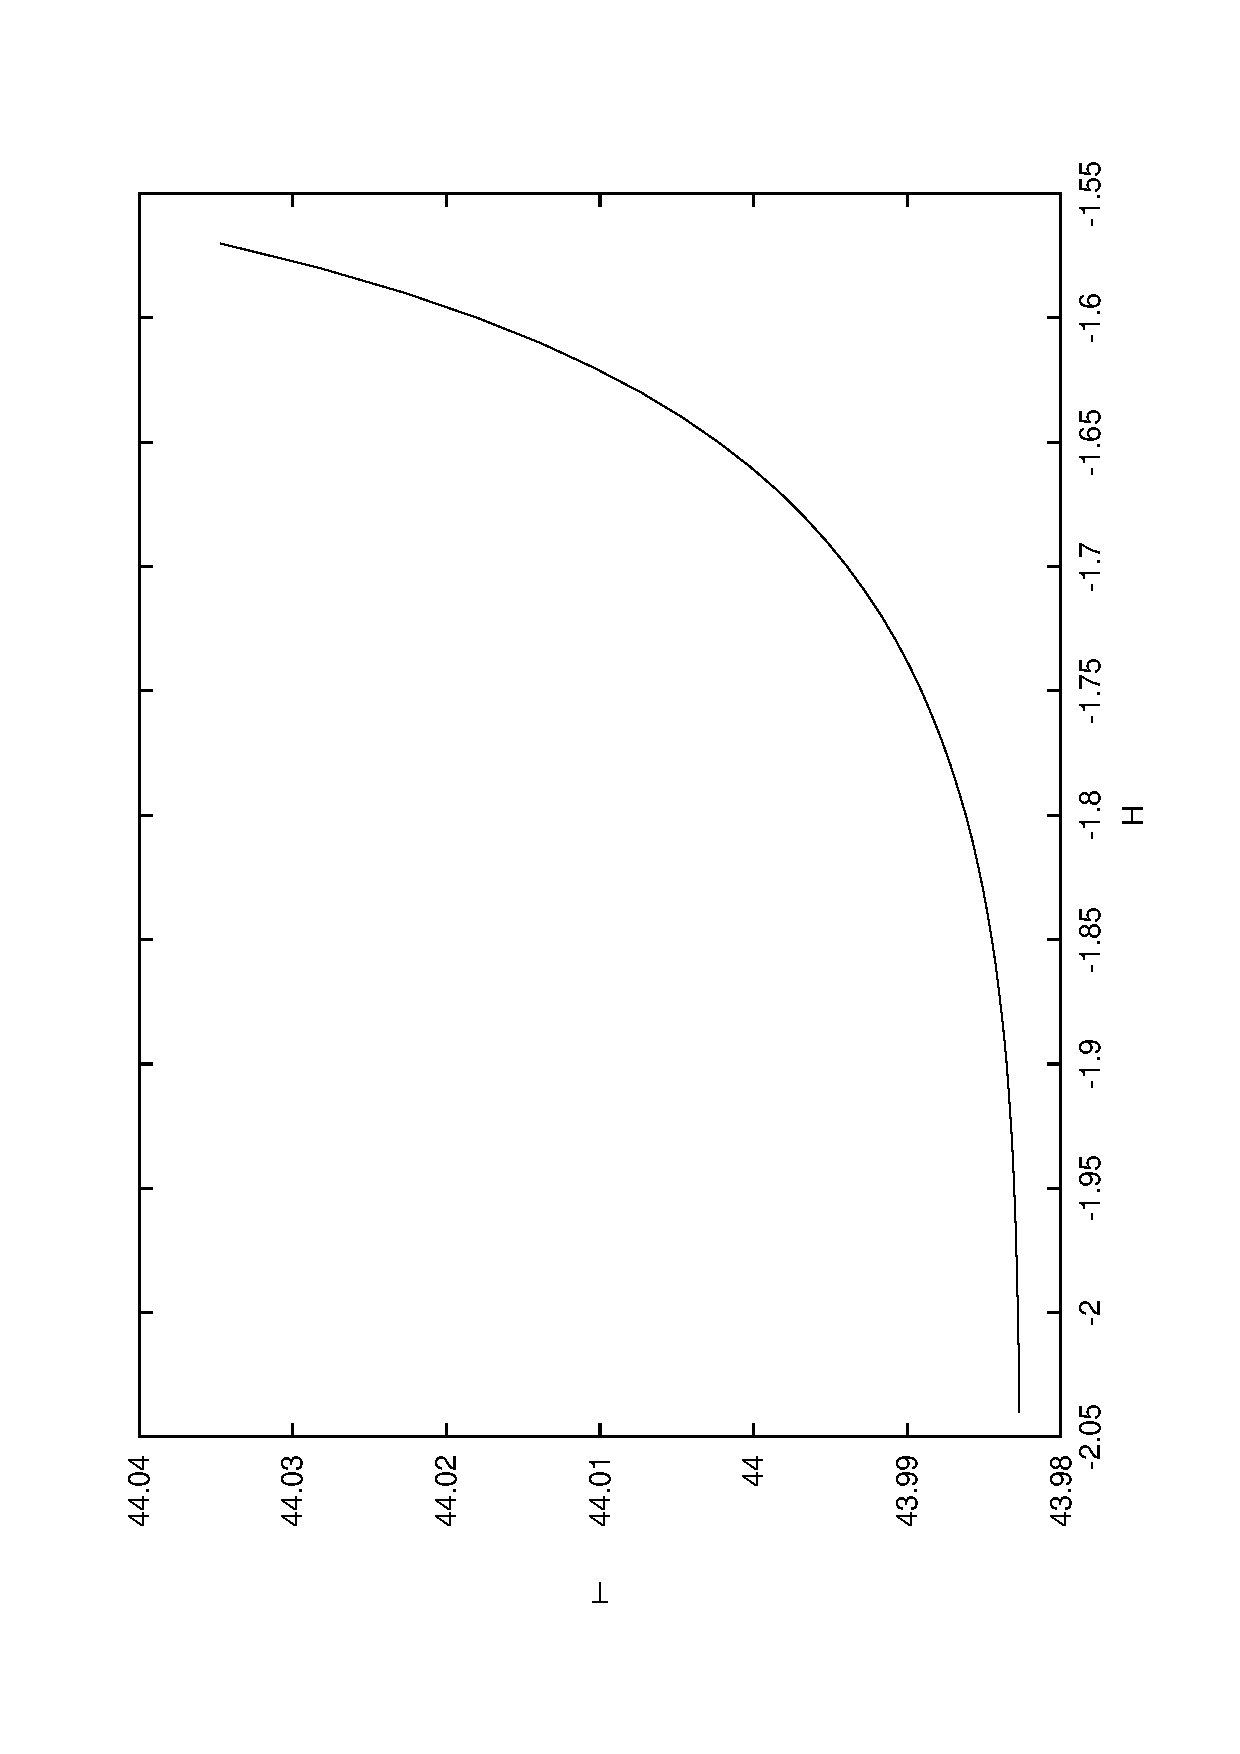
\includegraphics[angle=-90,width=\textwidth]{figs/porbits}
\caption{Resonant family of periodic orbits. 
We show period $T$ as a function of energy level $H$.}
\label{fig:porbits}
\end{figure}

Finally, we have also investigated other energy levels for the
existence of a periodic orbit, and the dependence of the period $T(H)$
with respect to the energy level $H$. We obtain the results shown in
figure~\ref{fig:porbits}.

Let $H_-=-2.04$ and $H_+=-1.57$.
For all energy levels $H\in [H_-,H_+]$, the Newton method converges
and we are able to find a periodic orbit with high accuracy.

As seen in figure~\ref{fig:porbits}, period $T(H)$ increases with energy $H$.
Notice that period tends to $14\pi=43.982\dots$ as energy tends to the
endpoint $H_-$.

\begin{figure}
\subincludefrom{figs/}{trtbp_porbits}
\caption{Extremal periodic orbits of the family: circular periodic
orbit with $H=H_-$ (in red), elliptical periodic orbit with $H=H_+$
(in green).}
\label{fig:trtbp_porbits}
\end{figure}

Let us plot the extremal periodic orbits of the family, i.e. the
orbits that correspond to the endpoints $H_-$ and $H_+$. See
figure~\ref{fig:trtbp_porbits}.
The extremal periodic orbit with $H=H_-$ is very circular, and it
passes far from Sun and Jupiter.
The extremal periodic orbit with $H=H_+$ is very elliptical, and it
passes very close to Jupiter (Jupiter orbits the circle of radius 1).
In fact, the Newton method probably fails to converge past $H_+$ due
to the fact that the periodic orbits tend to the asymptotic manifolds
$W^{u/s}(L_2)$ of the collinear equilibrium point $L_2$.

\begin{figure}
\subincludefrom{figs/}{Ldeviation}
\caption{Maximum deviation of the square of semi-major axis $L$ with
respect to the resonant value $7^{1/3}$, see
equation~\eqref{eq:Ldeviation}.}
\label{fig:Ldeviation}
\end{figure}

We want to verify that the family of periodic orbits is close to the
resonance, i.e. that the $L$ component stays close to the value
$7^{1/3}$.
Let $\gamma_H$ be the periodic orbit with energy level $H$.
Integrating the periodic orbit in Delaunay coordinates
$\gamma_H(t)=(l(t),L(t),g(t),G(t))$ over one period $T_H$, we compute
the quantity 
\begin{equation} \label{eq:Ldeviation}
 L_{\max}(H) = \max_{t \in [0,T_H)} |L(t)-7^{1/3}|.
\end{equation}
The function $L_{\max}(H)$ is plotted in figure~\ref{fig:Ldeviation}.
Notice that we obtain $|L(t)-7^{1/3}| < 7\mu$ for all $t\in \RR$.

\section{Hyperbolic Splitting}\label{sec:hyperbolic_splitting}

In this section, we compute the hyperbolic splitting associated to the
resonant family of periodic orbits, i.e. to the NHIM.

First we consider the periodic orbit $\Gamma$ with $H=-1.6$ that we
found in section~\ref{sec:periodic_orbit}.
Specifically, we will work with the periodic orbit corresponding to the fixed
point 
\[ p^*=(x,p_x)=(1.298\dots,0), \]
of the iterated Poincare map $\sixmap$.

%%%%%%%%%%%%%%%%%%%% COMMENTED OUT %%%%%%%%%%%%%%%%%%%%%%%%%
\begin{comment}

Firstly, we use the energy condition~\eqref{eq:energy} to derive the momentum
$p_y$ of the periodic orbit from the fixed energy level $H$.

\begin{verbatim}
roldan@pollo:~/research/splitting/hinv$ hinv
0.95387536e-3                                    #input: mu 
-1.6                                             #input: H
1.298584116092567e+00 0 0 0                      #input: (x,y,p_x)
1.124715918064501e+00                            #output: p_y
\end{verbatim}

Thus the periodic orbit passes through the point
\[ p^* =(x,y,p_x,p_y) = (1.298\dots,0,0,1.124\dots). \]

Next we compute the 4D derivative of the Poincare map evaluated at $p$.
\begin{verbatim}
roldan@pollo:~/research/splitting/dprtbp$ ./dprtbp
0.95387536e-3                                    #input: mu
12                                               #input: number of iterates

#input: p=(x,y,p_x,p_y)
1.302517353445867e+00 0.0 -3.020227156619462e-14 1.123521120789039e+00

#output: DP(p)
 9.432107872646583e-01  4.884454006866669e-04  1.638463890442024e-04 -1.081239670346104e-01
-3.197361827930326e+02  1.322330288965648e+00  1.081239678263585e-01 -6.087618144610592e+02
 1.679339627032353e+02 -1.692953362066567e-01  9.432107868487905e-01  3.197361827930314e+02
 1.692953362048959e-01 -1.456113305108453e-03 -4.884454011034487e-04  1.322330288962255e+00
\end{verbatim}

We compute the characteristic multipliers of the variational equation along
$\Gamma$, i.e. the eigenvalues/eigenvectors of the previous matrix.

\begin{verbatim}
octave:1> M = [
>  9.432107872646583e-01,  4.884454006866669e-04,  1.638463890442024e-04, -1.081239670346104e-01;
> -3.197361827930326e+02,  1.322330288965648e+00,  1.081239678263585e-01, -6.087618144610592e+02;
>  1.679339627032353e+02, -1.692953362066567e-01,  9.432107868487905e-01,  3.197361827930314e+02;
>  1.692953362048959e-01, -1.456113305108453e-03, -4.884454011034487e-04,  1.322330288962255e+00 ];
octave:2> # Compute eigenvectors/eigenvalues
octave:2> [evects, evals] = eig(M);
octave:3> format long
octave:4> # Eigenvalues:
octave:4> diag(evals)
ans =

  2.041166124027443 + 0.000000000000000i
  0.489916028013873 + 0.000000000000000i
  1.000000000000019 + 0.000000048832101i
  1.000000000000019 - 0.000000048832101i

octave:5> # Eigenvectors:
octave:5> evects
evects =

 Columns 1 and 2:

   0.000459296287307 + 0.000000000000000i   0.000459296288459 + 0.000000000000000i
   0.885315650974952 + 0.000000000000000i  -0.885315650974949 + 0.000000000000000i
  -0.464988292790554 + 0.000000000000000i   0.464988292790560 + 0.000000000000000i
  -0.001369216360726 + 0.000000000000000i  -0.001369216360732 + 0.000000000000000i

 Columns 3 and 4:

   0.000000000015563 + 0.000041665118829i   0.000000000015563 - 0.000041665118829i
  -0.318028715581940 + 0.000000000000001i  -0.318028715581940 - 0.000000000000001i
   0.948081079787184 + 0.000000000000000i   0.948081079787184 - 0.000000000000000i
  -0.000000000007558 - 0.000021883485796i  -0.000000000007558 + 0.000021883485796i

\end{verbatim}

As expected, there are two real eigenvalues
and two complex eigenvalues of modulus (approximately) 1. 

One eigenvalue of modulus 1 corresponds to the tangent direction to the
periodic orbit, and due to symplecticity of the flow there is another
eigenvalue of modulus 1. The corresponding eigenvectors (columns 3 and 4 of
matrix "evects") should span the tangent space to the family of periodic orbits
at $p$. 
%Notice that the corresponding eigenvectors
%(columns 3 and 4 of matrix "v") are almost pendicular to the Poincare
%section
%$\{y=0\}$, as expected.

As a test, we compute the product of the two couples of eigenvalues.
Due to symplecticity, the product should be 1 in exact computations:

\begin{verbatim}
octave:6> 2.041166124027443*0.489916028013873
ans = 0.999999999999997
octave:7> (1.000000000000019 + 0.000000048832101i)*(1.000000000000019 - 0.000000048832101i)
ans = 1.00000000000004
\end{verbatim}

%Since
%\[ u_\xi(T(p),p)f(p) = f(u(T(p),p)) = f(p), \]
%$f(p)$ is an eigenvector of the fundamental matrix solution, with eigenvalue
%$1$. Indeed, the eigenvectors with eigenvalue $1$ that we found above agree
%up to a small error with the vector $f(p)$. Let us show this by computing
%$f(p)$:
%
%\begin{verbatim}
%roldan@pollo:~/research/splitting/frtbp$ ./rtbp 
%0.95387536e-3                                      #input: mu
%#input: p=(x,y,p_x,p_y):
%1.302517353445867e+00 0.0 3.173461397015698e-12 1.123521120789039e+00
%#output: f(p):
%3.173461397015698e-12 -1.789962326568280e-01 5.336088617968329e-01 -3.173461397015698e-12
%\end{verbatim}
%
%Comparing the vector $f(p)$ and the eigenvectors above (columns 3 or 4) we
%see that they differ (approximately) by a multiplicative constant.

%%%%%%%%%%%%%%%%%%%% END COMMENTED OUT %%%%%%%%%%%%%%%%%%%%%%%%%
\end{comment}

Next we compute the derivative of $\sixmap$ evaluated at $p^*$.
\begin{verbatim}
roldan@pollo:~/research/splitting/dprtbp$ dprtbp_2d 
0.95387536e-3                        #input: mu
-1.6                                 #input: H
6                                    #input: number of iterates 
1.298584116092567e+00 0              #input: p^*

#output: DP(x,p_x)
 1.1828184291e+01  3.7987648894e-02
 3.6566080689e+03  1.1828184278e+01
\end{verbatim}

We compute the characteristic multipliers of the variational equation along
$\Gamma$, i.e. the eigenvalues $\rho_u, \rho_s$ and eigenvectors $v_u,
v_s$ of the previous matrix.

\begin{verbatim}
roldan@pollo:~/research/splitting/hyper$ ./hyper 
0.95387536e-3 -1.6 6                # input: mu H iterates
1.298584116092567e+00 0             # input: p^*

output:
rho_u =  2.361402084615086e+01
rho_s =  4.234772241718499e-02
v_u = ( 3.223144271056768e-03,  9.999948056570134e-01)
v_s = (-3.223144267529246e-03,  9.999948056570247e-01)
\end{verbatim}

As a test, we compute the product of the two couples of eigenvalues.
Due to symplecticity, the product should be $1$ in exact computations:

\begin{verbatim}
roldan@pollo:~/research/splitting/hyper$ echo \
> '23.61402084615086*0.04234772241718499' |bc -l
.99999999994641643990
\end{verbatim}

Notice that, due to the symmetry with respect to the horizontal, the
eigenvectors should have the same entries (up to changes in sign).
This is indeed true up to the 10-th digit (compare vu[0] and vs[0]).

As expected, there are two real eigenvalues
\[ \rho_u = 23.61402084615086, \qquad \rho_s = 0.04234772241718499. \]
The stable and unstable eigenvectors $v_s, v_u$ (columns 1 and 2 of matrix
"evects") are tangent to the stable and unstable manifolds. 
%Notice that $v_u, v_s$, when projected
%to the $xy$ space, are almost parallel. This will give rise to
%unstable/stable manifolds with a small splitting angle.

Next we compute the hyperbolic splitting for the whole family of
periodic orbits.

\begin{verbatim}
roldan@pollo:~/research/splitting/hyper$ ./hypers <hypers.dat
>hypers.res
\end{verbatim}

\begin{figure}
\subincludefrom{figs/}{hypers}
\caption{Hyperbolic splitting associated to family of periodic orbits. 
We plot characteristic exponents $\lambda_u, \lambda_s$ as a function
of energy level $H$.}
\label{fig:hypers}
\end{figure}

Figure~\ref{fig:hypers} shows the characteristic exponents
$\lambda_u=log(\rho_u)$, $\lambda_s=log(\rho_s)$ of the periodic
orbits as a function of energy $H$.
Notice that the family loses hyperbolicity as $H\to H_-$.

\section{Invariant manifolds}\label{sec:invariant_manifolds}

In this section, we compute the stable and unstable invariant manifolds
associated to the periodic orbit $\Gamma$ with $H=-1.6$ that we found
in section~\ref{sec:periodic_orbit}.

Let us next compute the unstable manifold $W^u(p)$. 
Let $h$ be a small displacement in the unstable direction.
We will grow the manifold from the linear segment between the points $p+hv_u$
and $\sixmap(p+hv_u)$. We discretize the segment into a mesh of points and iterate
them by the Poincare map $\sixmap$.

%\begin{rem}
%In practice, we don't take a constant value for $h$. Instead, we choose $h$
%according to the strength of hyperbolicity. In particular, we take
%$h:=10^{-5}\lambda_s$.
%\end{rem}
 
Points in the unstable manifold are iterated forwards by the map $\sixmap$.
Points in the stable manifold are iterated backwards by the \emph{inverse} 
map $\sixmap^{-1}$.

We compute the unstable manifold, and save it to file "unstmfld.res".

\begin{verbatim}
roldan@pollo:~/research/splitting/invmfld$ ./invmfld >unstmfld.res
0.95387536e-3 -1.6                             #input: mu, H
6                                              #input: num. iterates
1.298584116092567e+00 0                        #input: p^*
3.223144271056768e-03  9.999948056570134e-01   #input: v_u
2.361402084615086e+01                          #input: rho_u
#input: desired "length" of manifold
6
0                                              #input: unstable flag

#output:
h: 1.000000e-06
Estimated error of manifold: 5.040421e-09
\end{verbatim}

The estimated error of the manifold is computed in the following way. Let
$\rho_u$ be the unstable eigenvalue, and $v_u$ the corresponding
eigenvector. Let $\sixmap$ be the Poincare map. Let $p$ be the fixed
point. If $h$ is a small displacement in the unstable direction, then 
\[ \sixmap(p+hv_u) = p+\rho_uhv_u + O(h^2). \]
The size of the term $O(h^2)$ can be estimated as
\[ ||\sixmap(p+hv_u)-p-\rho_uhv_u||. \]
Similarly, in the stable case,
\[ ||\sixmap^{-1}(p+hv_s)-p-\frac{1}{\rho_s}hv_s||. \]

\begin{rem}
In practice, we choose the small increment $h$ such that the estimated
error commited in the linear approximation of the manifold is
negligible (smaller than $10^{-11}$).
\end{rem}
 
\begin{figure}
\subincludefrom{figs/}{invmfld}
\caption{Invariant manifolds of the fixed point $p^*$: unstable in
red, stable in green. The fixed point is located at the bottom left
corner.}
\label{fig:invmfld}
\end{figure}

The unstable and stable manifolds of $p^*$ are plotted in
figure~\ref{fig:invmfld}. 
Notice that both manifolds have some sharp fold.
For clarity, we only grow the manifolds up to this fold.
We could of course grow a longer piece of the manifolds if desired.

\begin{figure}
\subincludefrom{figs/}{invmfld_it}
\caption{Invariant manifolds of the fixed points $p_0, p_1,\dots,p_5$.
(See text).
The fixed points are marked blue.}
\label{fig:invmfld_it}
\end{figure}

One can think of $p^*$ as a $6$-periodic point of the Poincare map
$P$, or as a fixed point of the iterated Poincare map $\sixmap=P^6$. 
Let $p_i=P^i(p^*)$ be the iterates of the fixed point $p^*$, for
$i=0,\dots,5$.
All iterates $p_i$ are also fixed points of $\sixmap$.
They have associated unstable and stable manifolds, which can be
obtained from $W^u(p_0), W^s(p_0)$ by iteration under $P$.
Figure~\ref{fig:invmfld_it} shows the manifolds of all iterates.

Notice that the dynamics of the asteroid, when at perihelion, is
reversible with respect to the $l=g=0$ angles in Delaunay variables. 
In rotating polar variables, the condition of being at the perihelion
implies $\dot r = 0$, and the $l=g=0$ condition translates to
$\phi=0$. 
Hence, in rotating eucliden variables, this implies $y=0$ and $\dot r
= p_x \cos \phi + p_y \sin \phi = 0$, so $p_x=0$.

In figure~\ref{fig:invmfld_it}, it is evident that the dynamics is
reversible with respect to the $p_x=0$ line (and we have $y=0$ because
we are on the poincare section).

Figure~\ref{fig:invmfld_it} shows that the manifolds do intersect
transversally at different homoclinic points. 
We are interested in measuring the splitting angle between the
manifolds.
Unfortunately, the homoclinic points do not lie on the reversibility
line $p_x=0$. This would be very useful in order to compute them.

In order to have the homoclinic points lie on the reversibility line,
we look at the manifolds on the new poincare section

\[ \Sigma ' = \{y=0,\ p_y<0\}. \]

First of all, we flow the point $p_0$ forwards to the section $\Sigma'$,
obtaining a point $p_0'\in \Sigma'$.

\begin{verbatim}
roldan@pollo:~/research/splitting/prtbp2$ sec1sec2 
0.95387536e-3                             #input: mu
-1.6                                      #input: H
1.298584116092567e+00 0.0                 #input: p_0

#output:
-1.600000e+00                                   # H
-3.221507692925773e+00 -3.757823611945582e-01   # p_0'
5.277795909553800e+00                           # integration time
\end{verbatim}

Then we iterate $p_0'$ twice to obtain $p_2'$:
\begin{verbatim}
roldan@pollo:~/research/splitting/prtbp2$ prtbp2_2d
0.95387536e-3 
-1.6 
2
-3.221507692925773e+00 -3.757823611945582e-01   #input: p_0'

#output:
-5.919861224972698e+00 -5.874500915770887e-02   #output: p_2'
1.345572139790225e+01
\end{verbatim}

Next we compute the hyperbolic splitting at $p_2'$.
\begin{verbatim}
roldan@pollo:~/research/splitting/hyper2$ hyper2
0.95387536e-3 
-1.6 
6 
-5.919861224972698e+00 -5.874500915770887e-02

output:
rho_u =  2.361402083322900e+01
rho_s =  4.234772244243862e-02
v_u = (-9.945079515089161e-01, -1.046610452152056e-01)
v_s = (-9.966659836858821e-01,  8.158993175296168e-02)
\end{verbatim}
Of course, the eigenvalues coincide with the eigenvalues previously
computed on the section $\Sigma'$ (see
section~\ref{sec:hyperbolic_splitting}).

\begin{figure}
\subincludefrom{figs/}{invmfld2}
\caption{Invariant manifolds on the section $\Sigma'$.}
\label{fig:invmfld2}
\end{figure}

\begin{figure}
\subincludefrom{figs/}{invmfld2_it23}
\caption{Invariant manifolds of the points $p_2$ and $p_3$ on the
section $\Sigma'$. Due to the symmetry, points that lie on the line
$p_x=0$ (marked in blue) are intersection points.}
\label{fig:invmfld2_it23}
\end{figure}

Finally we compute the invariant manifold structure on $\Sigma'$. See
figures~\ref{fig:invmfld2} and~\ref{fig:invmfld2_it23}.
Now the points of the manifolds that lie on the symmetry line $p_x=0$
are homoclinic points between $p_2$ and $p_3$.

\begin{rem}
By pure chance, for this energy value $H=-1.6$, the manifolds of $p_2$
and $p_3$ seem to have a secondary homoclinic tangency close to the
points $(-5.67,0.03)$ and $(-5.67,-0.03)$.
\end{rem}

\section{Homoclinic orbit}\label{sec:homoclinic_orbit}

\begin{figure}
\subincludefrom{figs/}{invmfld2_it23_H174}
\caption{Invariant manifolds of the points $p_2$ and $p_3$ for the
energy level $H=-1.74$.}
\label{fig:invmfld2_it23_H174}
\end{figure}

Let us now consider an energy level that is closer to the unperturbed
situation, e.g. $H=-1.74$. The corresponding manifolds are given in
figure~\ref{fig:invmfld2_it23_H174}.
In this section, we compute the intersection point $z$ of the
manifolds $W^u(p_3)$ and $W^s(p_2)$.

Notice that there are two intersection points, $z$ and $\hat z$,
corresponding to the ``inner'' and ``outer'' separatrices,
respectively.
For simplicity, we will only discuss the outer separatrix; the inner
one is treated analogously.

In general, there are uncountably many intersection points. 
For instance, in figure~\ref{fig:invmfld2_it23} we show $3$
intersections on the symmetry line for the outer separatrix.
However, in the unperturbed situation there is one distinguished 
intersection point located ``in the middle'' of the separatrix. 
We call it the ``primary'' intersection point.
This corresponds to the point $z$ in figure~\ref{fig:invmfld2_it23_H174}.
We will continue this primary intersection into a family of
intersection points $\{z_H\}$, as we vary energy.

For $H=-1.74$, the primary intersection point $z$ corresponds to the
``first'' intersection of the manifolds with the $p_x=0$ line (as we
grow the manifolds from the fix points).
Thanks to the symmetry, it is enough to look for the intersection of
$W^u(p_3)$ with the $p_x=0$ axis, because $W^s(p_2)$ must also
intersect the axis at the same point.

Let us explain the numerical method that we use to compute the
homoclinic point.
Let $p$ denote the fixed point $p_3'$ on the section $\Sigma'$.
Let $v_u$ be the unstable eigenvector associated to the point $p=p_3'$.
We consider the unstable fundamental segment $l_u$ between $p+hv_u$ and
$\sixmap(p+hv_u)$ defined in section~\ref{sec:invariant_manifolds}.

First of all, we look for the first natural $n$ such that the unstable
fundamental domain $\sixmap^n(l_u)$, intersects the $p_x=0$ axis.
For our example periodic orbit we need $n=15$ iterations:

\begin{verbatim}
roldan@pollo:~/research/splitting/approxint$ approxint
#input: mu, k, unst flag, axis line
0.95387536e-3 6 0 0.0        
-1.74                                           #input: H
-5.560849822624931e+00 5.681451293257738e-02    #input: p_3
-9.932197905794894e-01 -1.162516563375987e-01   #input: v_u
2.725168763316296e+00                           #input: rho_u

#output:
H: -1.740000e+00
Optimal displacement: 1.000000e-06
Estimated error of manifold: 1.267216e-12
Approximate interval: 6
Approximate splitting half-angle: 0.072504

#output:
-1.740000e+00                                  #output: H
15                                             #output: n
#output: (h1,h2) root enclosure
1.104555663946585e-06 1.121981607929951e-06    
-5.730939670475454e+00 8.640857000751058e-05   #output: z (approx)
\end{verbatim}

Then, we use a standard numerical method (bisection-like
one-dimensional root finding) to find a point $p_u$ in the fundamental
segment $l_u$ such that 
\[ \pi_{p_x}(P^{n}(p_u))=0. \] 
(Here, $\pi_{p_x}\colon \field{R}^2\to \field{R}$ is the projection onto the
$p_x$ component).

\begin{verbatim}
roldan@pollo:~/research/splitting/intersec$ intersec
#input: mu, unst flag, axis line
0.95387536e-3 0 0.0
-1.74                                           #input: H
-5.560849822624931e+00 5.681451293257738e-02    #input: p_3
-9.932197905794894e-01 -1.162516563375987e-01   #input: v_u
2.725168763316296e+00                           #input: rho_u
15                                              #input: n
1.104555663946585e-06 1.121981607929951e-06     #input: (h1,h2)

#output
iter =   0, [0.0000011, 0.0000011], root = 0.0000011, err(est) = 0.000000017425944
iter =   1, [0.0000011, 0.0000011], root = 0.0000011, err(est) = 0.000000007919931
...
iter =  10, [0.0000011, 0.0000011], root = 0.0000011, err(est) = 0.000000000000001
status = success
-1.740000e+00                                   #output: H
-5.560850927526564e+00 5.681438360909211e-02    #output: p_u
6.596509542858771e+02                           #output: t_u
-5.730945639843551e+00 1.256642155700267e-10    #output: z=P(p_u)
\end{verbatim}
Thus we obtain the homoclinic point $z$ in
figure~\ref{fig:invmfld2_it23_H174}.  As expected, $z$ is in the the
$p_x=0$ axis (within $10^{-10}$ tolerance).

\begin{figure}
\subincludefrom{figs/}{intersec}
\caption{Family of primary intersection points. For each energy level
$H$, we plot the $x$ coordinate of the intersection point $z=(x,p_x)$
(the $p_x$ coordinate is equal to zero). Notice that the family is
continuous.}
\label{fig:intersec}
\end{figure}

Finally, we vary energy $H$ and continue this intersection point into
the family of primary intersections. We plot this family in
figure~\ref{fig:intersec}.

\begin{rem}
Let us again consider the energy level $H=-1.6$ for a moment. 
Recall that in figure~\ref{fig:invmfld2_it23} there are $3$
intersections on the symmetry line for the upper separatrix.
According to figure~\ref{fig:intersec}, the \emph{primary}
intersection point has $x$ coordinate equal to $x(z)=-6.12\dots$. 
This corresponds to the third intersection (counting from the left) in
figure~\ref{fig:invmfld2_it23}.
\end{rem}

\section{Splitting Angle} \label{sec:splitting_angle}

In this section, we compute the splitting angle between the manifolds
$W^u(p_3)$ and $W^s(p_2)$ at the primary homoclinic point.
Again, we use the energy level $H=-1.74$ for illustrating the computations.
As found in section~\ref{sec:homoclinic_orbit}, let $z$ be the primary
homoclinic point, and let $p_u$ be the point in the unstable
fundamental segment that maps to $z$, i.e.  $\sixmap^{n}(p_u) = z$.

Consider the tangent vector $v_u$ to the manifold at $p_u$. (Recall
that at this point the linear approximation is good enough, so we can
take as $v_u$ the unstable eigenvector.) 
Multiply $v_u$ by the Jacobian of $\sixmap$ at the successive iterates
$\sixmap^{i}(p_u)$, for $i=0,...,n-1$.
This way, we obtain the tangent vector of the unstable manifold at
$z$. Let us denote this vector $w_u=(w_1,w_2)$. 
We normalize it to $||w_u||=1$.

\begin{figure}
\subincludefrom{figs/}{splitangle}
\caption{Magnification of figure~\ref{fig:invmfld2_it23_H174} at the
intersection point~$z$. We show the vectors $w_u, w_s$ tangent to the
unstable and stable manifolds at $z$. Splitting angle $\alpha$ is
the angle between $w_u$ and $w_s$.}
\label{fig:splitangle}
\end{figure}

Due to reversibility, the vector tangent to the stable manifold at $z$
is $w_s=(w_1,-w_2)$. See figure~\ref{fig:splitangle}. Notice that we
choose the tangent vectors with the appropriate orientation, i.e. with
the same orientation as the trajectories on the manifolds. 

Thus the oriented splitting angle between $w_u$ and $w_s$ is 
\[ \alpha = 2\arctan_2(-w_1,-w_2), \]
where $\arctan_2$ is the arctangent function of two variables, which
uses the signs of the two arguments to determine the sign of the
result.

\begin{rem}
From now on, we will restrict the range of energy values to
\[ H\in[-1.81,-1.56]=[H_-,H_+], \]
or equivalently the range of eccentricities to
\[ e\in[0.48,0.66]=[e_-,e_+]. \] 
This is the range where we can validate the accuracy of our
computations (see section~\ref{sec:accuracy_computations}).
Below e=0.48, splitting size becomes comparable to the numerical
error. 
Thus one must use more sophisticated numerical methods to show that
splitting is nonzero (multiple precision arithmetic, high-order
approximation of local invariant manifolds using normal forms or
parametrization method, etc.)
\end{rem}

In figure~\ref{fig:splittings} we plot the splitting angle associated
to the outer separatrix for $e\in[e_-,e_+]$ (in green).
The splitting angle is nonzero for all energy values except for a
discrete set.  The splitting angle oscillates around zero with
decreasing amplitude as $e\to e_-$. 

Numerically, we find that the zeros of the splitting angle are
contained in the intervals listed in table~\ref{tab:zeros_inner_outer}
(right column).

*** We could study the behavior of $\alpha$ to see how exactly how fast
does it decrease: as a power, as en exponential? ***

\subsection{Accuracy of the Computations}
\label{sec:accuracy_computations}

For small eccentricities, the splitting angle~$\alpha$ becomes very
small.
We need to check the validity of $\alpha$, making sure that the size
of (accumulated) numerical errors in the computation is smaller than
the size of $\alpha$.

The smallest splitting angle in figure~\ref{fig:splittings},
corresponding to $e=0.48$, is 
\[ \alpha(0.48)= -1.777970294158603 \times 10^{-5}. \]
We check the validity of $\alpha(0.48)$ by recomputing this angle using 
an alternative numerical method.
First we compute the intersection of the manifolds $W^u(p_3)$ and
$W^s(p_2)$ with the horizontal axis defined by
\[ p_x = \frac{j}{10^{5}} \]
for $j\in (-2,-1,1,2)$. 

\begin{table}
\begin{tabular}{|c|c|c|c|}
\hline
$p_x$ & $x^u$ & $x^s$ & $x^u-x^s$ \\
\hline
$-0.00002$ & $-5.481541931871417$ & $-5.481541932226887$ &
$0.000000000355470$ \\
$-0.00001$ & $-5.481541931790012$ & $-5.481541931967703$ &
$0.000000000177691$ \\
$0.00000$ & $-5.481541931822124$ & $-5.481541931822124$ &
$0.000000000000000$ \\
$0.00001$ & $-5.481541931967703$ & $-5.481541931790012$ &
$-0.000000000177691$ \\
$0.00002$ & $-5.481541932226887$ & $-5.481541931871417$ &
$-0.000000000355470$\\
\hline
\end{tabular}
\caption{Sampling of the manifolds $W^u(p_3)$ and $W^s(p_2)$ at
different values of $p_x$, and their difference (last column).}
\label{tab:differentiation}
\end{table}

In table~\ref{tab:differentiation} we tabulate the $x$ coordinate of
$W^u(p_3)$ and $W^s(p_2)$ on these axis, and their difference
$d=x^u-x^s$ gives the distance between the manifolds.
We apply numerical differentiation to the last column of this table,
using central differences centered at $z$ with step sizes $0.00002$
and $0.00004$, and obtain the values:
\[ d1 = \frac{d(0.00001) - d(-0.00001)}{0.00002} =
-0.0000177691.\]
\[ d2 = \frac{d(0.00002) - d(-0.00002)}{0.00004} =
-0.0000177735.\]
Finally, we use Richardson extrapolation and obtain:
\[ d = \frac{4 d1-d2}{3} = -0.00001776763333333333. \]
Thus, using this second method, we obtain the splitting angle
\[ \alpha(0.48) = atan(-0.00001776763333333333) =
-0.00001776763333146364. \]
Compare the splitting angle computed using the two methods. They
differ by approximately $10^{-8}$.
This gives an estimate of the numerical error commited in our
computation of the splitting angle.

\begin{figure}
\subincludefrom{figs/}{diffs}
\caption{Splitting angle $\alpha(H)$ and estimate of the numerical
error $err(H)$ as a function of energy level $H$.}
\label{fig:diffs}
\end{figure}

We repeat this test for a range of energies $H\in[-1.81,-1.8]$. 
In figure~\ref{fig:diffs}, we compare the splitting angle $\alpha(H)$
and the estimate of the numerical error $err(H)$. This error stays
below $10^{-7}$, and it is several orders of magnitude smaller than
the splitting angle. 
Therefore we are confident that the splitting angle has been accurately
computed in the range of eccentricities considered,
$[e_-,e_+]=[0.48,0.66]$.

\section{Inner splitting} \label{sec:inner_splitting}

Finally, let us consider the family of primary homoclinic
intersections ${\hat z}_H$ associated to the \emph{inner} separatrix. 
Proceeding in the same way as in sections~\ref{sec:homoclinic_orbit}
and~\ref{sec:splitting_angle}, we compute the splitting angle
associated to the inner separatrix.

\begin{figure}
\subincludefrom{figs/}{splittings}
\caption{Splitting angle associated to inner and outer separatrices
(in radians).}
\label{fig:splittings}
\end{figure}

\begin{table}
\begin{tabular}{|c|c|}
\hline
inner & outer \\
\hline
$ ( -1.695,-1.694 ) $ & $ ( -1.701,-1.700 ) $ \\
$ ( -1.726,-1.725 ) $ & $( -1.731,-1.730 ) $ \\
$ ( -1.756,-1.755 ) $ & $ ( -1.760,-1.759 ) $ \\
$ ( -1.781,-1.780 ) $ & $ ( -1.784,-1.783 ) $ \\
$ ( -1.802,-1.801 ) $ & $ ( -1.805,-1.804 ) $ \\
\hline
\end{tabular} 
\caption{Intervals containing the zeros of inner splitting (left
column) and outer splitting (right column).}
\label{tab:zeros_inner_outer}
\end{table}

The inner and outer splittings are very similar. See
figure~\ref{fig:splittings}.
However, they become zero at different values of $H$. See
table~\ref{tab:zeros_inner_outer}.

\section{Delaunay coordinates}

We have programmed the transformation to obtain rotating Delaunay
coordinates $(l,L,g,G)$ from rotating cartesian $(x,y,p_x,p_y)$.
For example, let us transform the fixed point $p_0$ corresponding to
periodic orbit with $H=-1.6$.

\begin{verbatim}
roldan@pollo:~/research/splitting/cardel$ ./cardel
0.95387536e-3                                     #input: mu
-1.6                                              #input: H
1.298584116092567e+00 0 0 1.124715918064501e+00   #input: (x,y,p_x,p_y)

#output: (l,L,g,G)
0.000000000000000e+00 1.906394680726033e+00       # l, L
0.000000000000000e+00 1.460538226315030e+00       # g, G
\end{verbatim}
Since $p_0$ is at the perihelion when $t=0$, it has Delaunay coordinates
$l=g=0$.

Next we have programmed the vector field of the RTBP in Delaunay
coordinates.

*** Write down equations of RTBP in Delaunay coordinates. 
These are quite cumbersome expressions! 
Moreover, we have to deduce eccentricy $u$ numerically. 
Also, there is a trick by Vadim to determine the sign of $u$. ***

For instance, we compute the vector field at the fixed point $p_0$
corresponding to the periodic orbit with $H=-1.6$.

\begin{verbatim}
roldan@pollo:~/research/splitting/rtbp_del$ ./rtbpdel
0.95387536e-3                                 #input: mu
#input: p_0
0.000000000000000e+00 1.906394680726033e+00   # l, L
0.000000000000000e+00 1.460538226315030e+00   # g, G

#output: d/dt(l,L,g,G)
1.408489723196100e-01 -0.000000000000000e+00  #d/dt(l,L)
-9.791011070652882e-01 -0.000000000000000e+00 #d/dt(g,G)
\end{verbatim}
Since $p_0$ is at the perihelion when $t=0$, the derivatives of $L$
(square of semimajor axis) and $G$ (angular momentum) are zero.

To test the correctness of the vectorfield, we compare each component
to the corresponding partial derivative of the Hamiltonian function.
The partial derivative is computed numerically using a central
differences squeme.

\begin{verbatim}
roldan@pollo:~/research/splitting/rtbp_del$ ./rtbpdel_test 
0.95387536e-3                                 #input: mu
#input: p_0
0.000000000000000e+00 1.906394680726033e+00   # l, L
0.000000000000000e+00 1.460538226315030e+00   # g, G

#output: numerical derivatives versus analytical derivatives
L = 1.906395e+00
dot l = H'(L) = 0.1408489720 +/- 0.0000000235 # numerical
dot l = y[0] = 0.1408489723                   # analytical

l = 0.000000e+00
dot L = -H'(l) = 0.0000000002 +/- 0.0000000215
dot L = y[1] = -0.0000000000

G = 1.460538e+00
dot g = H'(G) = -0.9791011052 +/- 0.0000000262
dot g = y[2] = -0.9791011071

g = 0.000000e+00
dot G = -H'(g) = -0.0000000008 +/- 0.0000000221
dot G = y[3] = -0.0000000000
\end{verbatim}
Notice that the difference between the analytical and numerical
derivatives is smaller than the estimated numerical error (written
after the $\pm$ sign).

Next we have programmed the flow of the RTBP in Delaunay coordinates.
For example, we compute the flow at the periodic point $p_0$ after
time $T=44.01796898996710$ (the period of the periodic orbit, as
computed in section~\ref{sec:periodic_orbit}).
\begin{verbatim}
roldan@pollo:~/research/splitting/frtbp_del$ frtbpdel 
#input:
0.95387536e-3 
44.01796898996710
0.000000000000000e+00 1.906394680726033e+00
0.000000000000000e+00 1.460538226315030e+00

#output:
6.283185307179695e+00 1.906394680725900e+00 
-4.398229715025703e+01 1.460538226315012e+00
\end{verbatim}
Since this is a periodic orbit, the final condition has coords 
\[ \Phi_T(p_0) = (l=2\pi,\ L,\ g=-14\pi,\ G). \]

Finally, consider the poincare section 
\[ \Sigma_g=\{g=0\}, \]
and let $P_g\colon \Sigma_g \to \Sigma_g$ be the associated Poincare
map. 
Equivalently, if $g$ was considered as ``time'', $P_g$ would be the
time-$2\pi$ map, or stroboscopic map.
Notice that, in the rotating Delaunay variables, a $7:1$ resonant
periodic orbit crosses the section $\Sigma_g$ precisely $7$ times.

For example, we compute the $7$-th iterate of $p_0$ under the
poincare map $P_g$. 
\begin{verbatim}
roldan@pollo:~/research/splitting/prtbp_del$ ./prtbpdel
0.95387536e-3 7                               #input: mu, iterates
#intpu: p_0
0.000000000000000e+00 1.906394680726033e+00   # l, L
0.000000000000000e+00 1.460538226315030e+00   # g, G

#output: P_g^{7}(p_0)
9.947598300641403e-14 1.906394680725914e+00   # l, L
0.000000000000000e+00 1.460538226315020e+00   # g, G
4.401796898996748e+01                         # integration time
\end{verbatim}
Since this is a periodic orbit, the final condition has coords 
\[ P_g^{7}(p_0) = (l=2\pi,\ L,\ g=-14\pi,\ G). \]
Notice that the period of the periodic orbit $T=44.017\dots$ agrees
with the one computed in section~\ref{sec:periodic_orbit} using
euclidean coordinates.

Similarly, we can compute the inverse poincare map $P_g^{-1}$.

\section{Resonance structure}\label{sec:resonance_structure}

To better describe the resonance structure, we plot the manifolds
using Delaunay variables. 
Consider the fixed point $p_0$ corresponding to the periodic orbit
with $H=-1.6$.

First, we obtain the unstable and stable invariant manifolds of the
point $p_0$, and transform them to Delaunay variables. 
Notice that the transformed invariant manifolds do not lie on the
$\Sigma_g=\{g=0\}$ section.
Thus we apply the Delaunay flow to each point in the invariant
manifolds until it lies on the $\Sigma_g$ section.

To obtain the manifolds of all fixed points, We iterate the invariant manifolds
of $p_0$ by the Poincare map $P_g$ $7$ times.
\begin{verbatim}
roldan@pollo:~/research/splitting/doc/figs$ ./orbitpdel
<unstmfld_it0.dat >unstmfld_it0.res
\end{verbatim}

\begin{figure}
\subincludefrom{figs/}{orbitpdel}
\caption{Invariant manifolds in Delaunay variables.}
\label{fig:orbitpdel}
\end{figure}

\begin{figure}
\subincludefrom{figs/}{invmflddel}
\caption{Invariant manifolds in Delaunay variables (zoom).}
\label{fig:invmflddel}
\end{figure}

Figures~\ref{fig:orbitpdel} and~\ref{fig:invmflddel} show the
manifolds in Delaunay variables, on the $\Sigma_g$ section.
The manifolds ``look like'' those of a perturbed pendulum.

The fixed points $p_0$, $p_1$, \dots, $p_6$ are \emph{almost} (but not exactly)
equidistributed on the $l$ axis.
This is natural since the $\mu=0$ circular resonant periodic orbit
crosses the $\Sigma_0=\{g=0\}$ section every $l=2\pi k/14$ for
$k=0,\dots,6$.

Similarly, the invariant manifold structure is almost (but not
exactly) repeated every $2\pi/7=0.897\dots$.

The manifold structure is symmetrical with respect to the vertical
lines $l=0$ and $l=\pi$.

*** TO DO ***

We should also plot the resonant periodic orbit that we studied in the
beginning of this work. 
The associated manifolds look like a figure-eight inside the pendulum.

*** TO DO ***

\section{Reduced flow of the circular problem}

The program \emph{frtbpred} computes the time-$s$ reduced flow of
the circular problam. As a test, we integrate the initial condition
corresponding to the periodic orbit for time exactly $s=14\pi$.

\begin{verbatim}
roldan@pollo:~/research/splitting/frtbp_red$ frtbpred 
0.95387536e-3 
43.98229715025710533816                      # input: int.time s=14\pi
# input: initial condition x=(l,L,g,G,t,I)
0.000000000000000e+00 1.906394680726033e+00  
0.000000000000000e+00 1.460538226315030e+00
0 0

# output: final condition \phi(s,x)=(l,L,g,G,t,I)
-6.283185307179716e+00 1.906394680725890e+00 
4.398229715025710e+01 1.460538226315010e+00 
-4.401796898996715e+01 0.000000000000000e+00
\end{verbatim}
As expected, the final condition has coords 
\[ \phi(s,x) = (l=-2\pi,\ L,\ g=14\pi,\ G,\ t=-(14\pi+\mu T_0),\ I). \]
In particular, note that $t$ coincides with the period of the periodic
orbit in the old time.

\section{Inner and outer dynamics of the circular problem}

\subsection{Inner dynamics}

For the circular problem, the invariant cylinder is foliated by
periodic orbits.
According to Marcel's notes, the inner map for the circular problem is
given by

\[ F_0^{in}\colon\ (I,t)\to (I, t+\mu T_0(I)). \]

Here, $\mu T_0(I)$ is the period of the periodic orbit (modulo $2\pi$) in
the original time $t$.
Recall that we computed the periodic orbit as well as its period in
section~\ref{sec:symmetric_periodic_orbits}.
We plot the period $\mu T_0(H)$ as a function of energy level $H$ in
figure~\ref{fig:inner_circ}.

\begin{figure}
\subincludefrom{figs/}{inner_circ}
\caption{Shift $\mu T_0$ of the inner map, as a function of energy level $H$.}
\label{fig:inner_circ}
\end{figure}

The derivative of the function $\mu T_0(H)$ is clearly nonzero.
This means that the inner map is twist (and thus one can apply KAM
theorem).

As an extra test, we compute the same shift $\mu T_0$ for a specific
energy level $H=-1.6$ using two different methods. First by computing
the period of the periodic orbit. The period was computed in
section~\ref{sec:symmetric_periodic_orbits}, and it is $2\times
2.200898449498355e+01 = 4.401796898996710e+01$. Thus the shift is
\[ \mu T_0(-1.6) = 44.01796898996710e+01 \mod 14\pi =
.03567183970999466184. \]

Then by computing the integral expression in Marcel's notes using
numerical integration:
\begin{verbatim}
roldan@pollo:~/research/splitting/inner_circ$ ./inner_circ <inner_circ.dat 

# output: 
estimated error =  5.347e-13
3.567183971001953e-02           # \mu T_0
\end{verbatim}
The difference in computing the shift using both methods is of the order
$10^{-10}$.

\subsection{Outer dynamics}

According to Marcel's notes, the outer map for the circular problem is
given by

\[ F_0^{out}\colon\ (I,t)\to (I, t+\mu \omega_0(I)), \]

where

\[ \omega_0(I) = -\omega_0^-(I) -\omega_0^+(I). \]

Let us explain how we compute $\omega_0^+$. Fix $(H_0=-1.74,t_0=0)$,
that is the level of energy and initial condition in $t$. 
Recall that in section~\ref{sec:homoclinic_orbit} we obtained a
primary homoclinic point which belongs to the Poincare section
$\Sigma'$. 

We transform this homoclinic point from Cartesian variables to
Delaunay. From now on, we work with the reduced flow in Delaunay
coordinates for the circular problem. 

\begin{verbatim}
roldan@pollo:~/research/splitting/cardel2$ cardel2_2d 
0.95387536e-3                                 #input: mu
-1.74                                         #input: H
-5.730945639853097e+00 0                      #input: z=(x,p_x)

#output: z=(l_h, L_h, g_h, G_h)
3.141592653589793e+00 1.922442586446909e+00  # l_h, L_h
6.283185307179586e+00 1.604706451008939e+00  # g_h, G_h
\end{verbatim}
Notice that, due to reversibility, the homoclinic point has
$g_h=2\pi=0$, so it is precisely on the section $g=0$. 
THIS IS PERFECT, because we don't need to flow it forwards until it
reaches the section $g=0$.

We would like to take the extended point $(l_h, L_h, 0, G_h, t_0)$ and
flow it from $s=0$ until $s=14 N\pi$, for a certain (big) natural $N$. 
Then we would obtain a new point $(l_h^+, L_h^+, 0, G_h^+, t_1)$ which
is very close to the cylinder.

Numerically, however, forward integration along the stable manifold
leads to amplification of errors.
In practice, we arrange this computation as backward integration.
We consider the point $p_u$ that we found in
section~\ref{sec:homoclinic_orbit}. 
Recall that $p_u$ is in the unstable manifold of the non-reduced flow,
very close to the cylinder. 
Equivalently, it is in the \emph{stable} manifold for the reduced
flow. Thus let us rename the point by $p_s$.
Notice that $p_s$ is not in the section $g=0$.
\begin{verbatim}
roldan@pollo:~/research/splitting/cardel2$ cardel2_2d 
0.95387536e-3
-1.74
-5.560872184178592e+00 5.681189561885759e-02   #input: p_s = (x,p_x)

#output: p_s=(l,L,g,G)
3.614415602587796e+00 1.912860780992552e+00    # l, L
6.115377037688049e+00 1.603347301832497e+00    # g, G
\end{verbatim}
We flow $p_s$ backwards (by the reduced flow) until it reaches the
section $g=0$. 
Thus, we obtain a different point, with coordinates $(l_h^+, L_h^+, 0,
G_h^+)$, that is close to $p_s$. 
Take the extended point $(l_h^+, L_h^+, 0, G_h^+, t_0)$ and
flow it \emph{backwards} from $s=0$ until $s=-14 N\pi$, for a certain
(big) natural $N$.
Then we obtain the homoclinic point $(l_h, L_h, 0, G_h, -t_1)$ in the
section $g=0$.

\begin{rem}
We take $t_1$ modulo $2\pi$.
\end{rem}

As explained in Marcel's notes, from the definition of the inner map
it follows that $t_2 = t_1 +N\mu T_0$.
Finally, the function $\omega_0^+$ is simply $\omega_0^+ = t_2 - t_0$.

Analogously, we can find $\omega_0^-$.

\begin{figure}
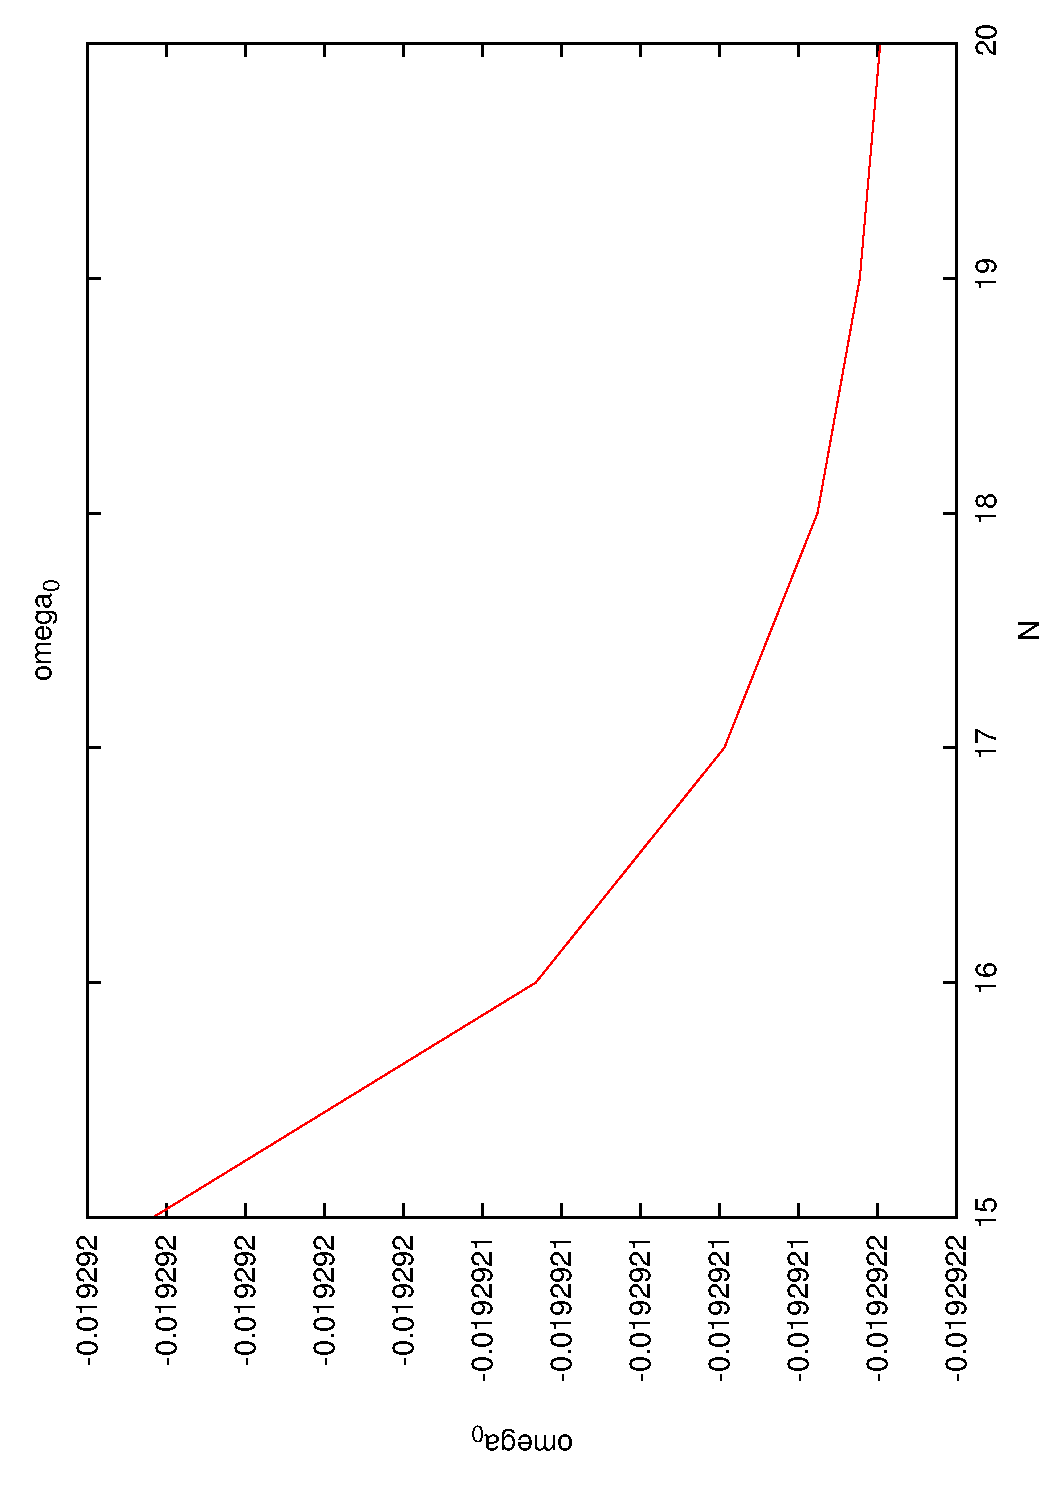
\includegraphics[angle=-90,width=\textwidth]{figs/omega}
\caption{Convergence of $\omega_0$ as a function of the number of
iterates $N$ along the homoclinic orbit.}
\label{fig:omega}
\end{figure}

As a test, we consider a fixed value of energy $H=-1.6$, and we
compute the value of $\omega_0$ for different number of iterates $N$.
See figure~\ref{fig:omega}.
As expected, $\omega_0$ has order $\mu$, and it converges to an
asymptotic value as $N$ increases.

\begin{figure}
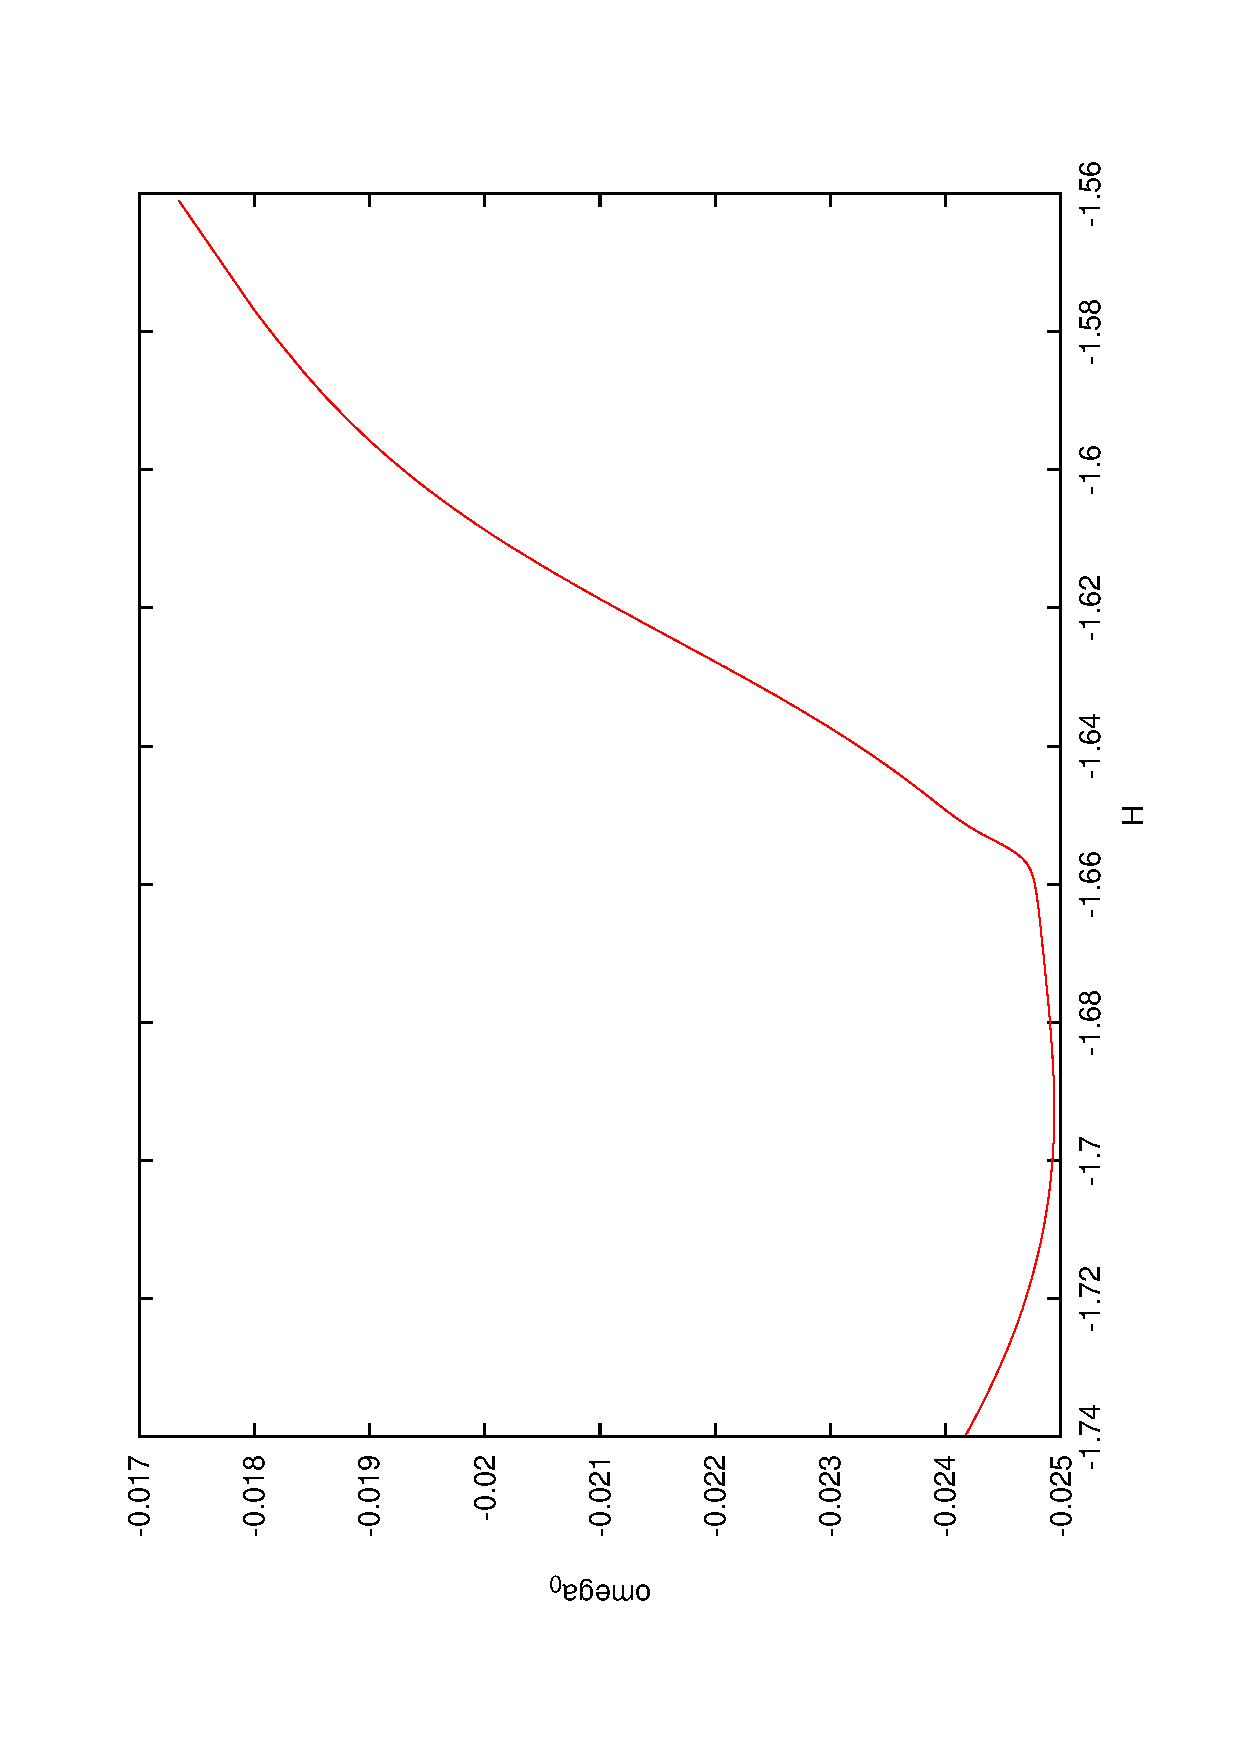
\includegraphics[angle=-90,width=\textwidth]{figs/omegas}
\caption{Shift $\omega_0$ of the outer map, as a function of energy
level $H$.}
\label{fig:omegas}
\end{figure}

Finally, we compute $\omega_0$ as a function of energy $H$. The
result is shown in figure~\ref{fig:omegas}.

A helpful test to verify that the function $\omega_0^+$ is correct is
to check that indeed, the homoclinic orbit and the periodic orbit
converge
\[ dist^+(s) \equiv |\Phi_s(l_h,L_h,0,G_h,t_0) -
\Phi_s(l_p,L_p,0,G_p,t_0+\omega_0^+)| \xrightarrow{s\to\infty} 0 \]
with exponential decay. We have performed this test for values of the
energy in the range $[-1.74,-1.56]$. 

\begin{figure}
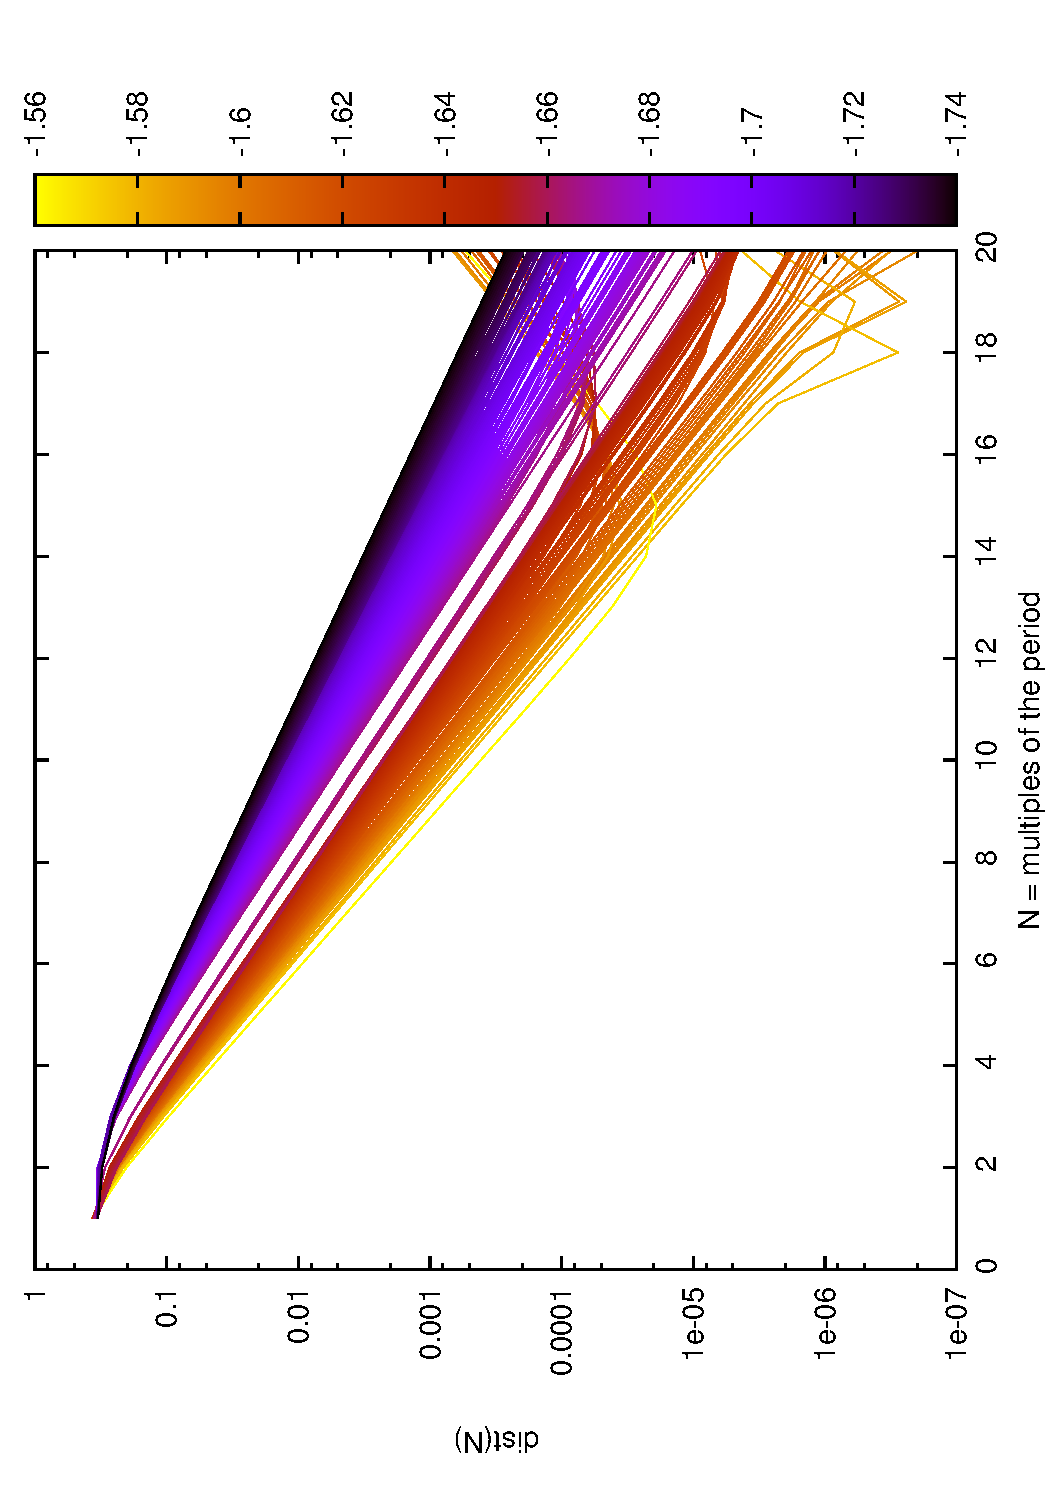
\includegraphics[angle=-90,width=\textwidth]{figs/omega_test}
\caption{Exponential decay of the function $dist^+$ as a function of
$N$ (multiples of the period) for different energy levels
$H\in[-1.74,-1.56]$.}
\label{fig:omega_test}
\end{figure}

The result of the test is shown in figure~\ref{fig:omega_test}.
Notice that the vertical axis is in logarithmic scale.
Let $s=14N\pi$. We plot the function $dist^+$ as a function of $N$
(multiples of the period).
The test shows exponential decay of the distance function for $s\leq
14\cdot(14\pi) \approx 600$.
For most energies, there is exponential decay up to time $s = 20\cdot
(14\pi) \approx 880$.

Recall that the periodic orbit becomes more hyperbolic as energy $H$
increases. Thus, the rate of exponential convergence between the
homoclinic orbit and periodic orbit increases as $H$ increases.
This is in accordance to figure~\ref{fig:omega_test}.

We have also performed the same test for $\omega_0^-$, and we have
verified that
\[ dist^-(s) \equiv |\Phi_s(l_h,L_h,0,G_h,t_0) -
\Phi_s(l_p,L_p,0,G_p,t_0-\omega_0^-)| \xrightarrow{s\to -\infty} 0 \]
with exponential decay.

\section{Inner and outer dynamics of the elliptic problem}

\subsection{Inner dynamics}

We study the inner map of the elliptic problem. From Marcel's notes,
we want to compute the first order of the $I$ component
\[ A_1(I,t) = A_1^+(I,t)e^{it} + A_1^-(I,t)e^{-it}. \]
Since $A_1^+$ and $A_1^-$ are complex conjugate,
\[ A_1(I,t) = 2\Re(A_1^+)\cos(t) - 2\Im(A_1^+)\sin(t). \]

Let us define the complex function
\begin{equation} \label{eq:f}
f(l,L,g,G) = \frac{\partial_t \Delta H_{ell}^{1,+}(l,L,g,G)}
      {-1+\mu\partial_G \Delta H_{circ}(l,L,g,G)}.
\end{equation}
We need to compute the complex integral $A^+(I)$ in Marcel's notes
\[ A^+(I) = -\mu\int_0^{-14\pi} f(\Phi_s(l_p,L_p,0,G_p)) e^{it(s)} ds, \]
where $\Phi_s$ denotes the flow of the reduced system, and
$(l_p,L_p,0,G_p)$ is the periodic point on the section $g=0$.

Notice that the denominator of $f$ is the same one used for the inner
dynamics of the circular problem.
Next we compute the numerator explicitly.
Let 
\begin{equation} \label{eq:DHell}
\Delta H_{ell}^1(l,L,g,G,t) = 
\frac{1-\mu}{\mu^2} B_1(-\frac{r}{\mu},v,g-t,t) 
-\frac{1}{1-\mu} B_1(\frac{r}{1-\mu},v,g-t,t),
\end{equation}
where
\begin{align*} 
B_1(r,v,g-t,t) &= -\frac{1}{2\Delta^3(r,v,g)}(2\cos t
-3r\cos(v+g+t)+r\cos(v+g-t)), \\
\Delta(r,v,g) &= (r^2+1-2r\cos(v+g))^{1/2}.
\end{align*}

\begin{rem}
In equation~\eqref{eq:DHell}, we follow Marcel and Vadim's convention
to place the large mass (Sun) to the left of the origin, and the small
mass (Jupiter) to the right.
In the code, however, we follow the astrodynamics convention to place
the large mass (Sun) to the right of the origin, and the small mass
(Jupiter) to the left. The only difference would be the terms
$B_1(\frac{r}{\mu},v,g-t,t)$ and $B_1(-\frac{r}{1-\mu},v,g-t,t)$.
We should probably stick to one convention.
\end{rem}

We write $B_1$ as a sum of harmonics
\begin{align*}
B_1(r,v+g,t) 
   &=-\frac{1-r\cos(v+g)-i2r\sin(v+g)}{2\Delta^3(r,v+g)}e^{it}
-\frac{1-r\cos(v+g)+i2r\sin(v+g)}{2\Delta^3(r,v+g)}e^{-it} \\
   &\equiv B_1^+(r,v+g)e^{it}+B_1^-(r,v+g)e^{-it}.
\end{align*}
Thus we have
\[ B_1^+(r,v+g) \equiv
-\frac{1-r\cos(v+g)-i2r\sin(v+g)}{2\Delta^3(r,v+g)}. \]

Taking partial derivatives with respect to $t$ we obtain
\[ \partial_t \Delta H_{ell}^1 = 
   \frac{1-\mu}{\mu^2} \partial_t B_1(-\frac{r}{\mu},v,g-t,t)
   -\frac{1}{1-\mu} \partial_t B_1(\frac{r}{1-\mu},v,g-t,t), \]
with
\[ \partial_t B_1(r,v+g,t) =
iB_1^+(r,v+g)e^{it}-iB_1^-(r,v+g)e^{-it}.\]

Putting it all together,
\begin{align*} 
\partial_t \Delta H_{ell}^1 
   &= \frac{1-\mu}{\mu^2} 
   \left[ iB_1^+(-\frac{r}{\mu},v+g)e^{it} -
      iB_1^-(-\frac{r}{\mu},v+g)e^{-it} \right] \\
   &-\frac{1}{1-\mu} 
   \left[ iB_1^+(\frac{r}{1-\mu},v+g)e^{it} -
      iB_1^-(\frac{r}{1-\mu},v+g)e^{-it} \right] \\
   &\equiv \partial_t \Delta H_{ell}^{1,+} e^{it} +
      \partial_t \Delta H_{ell}^{1,-} e^{-it}.
\end{align*}
Therefore we have
\[ \partial_t \Delta H_{ell}^{1,+} = 
\frac{1-\mu}{\mu^2} iB_1^+(-\frac{r}{\mu},v+g) -\frac{1}{1-\mu}
iB_1^+(\frac{r}{1-\mu},v+g). \]

\begin{figure}
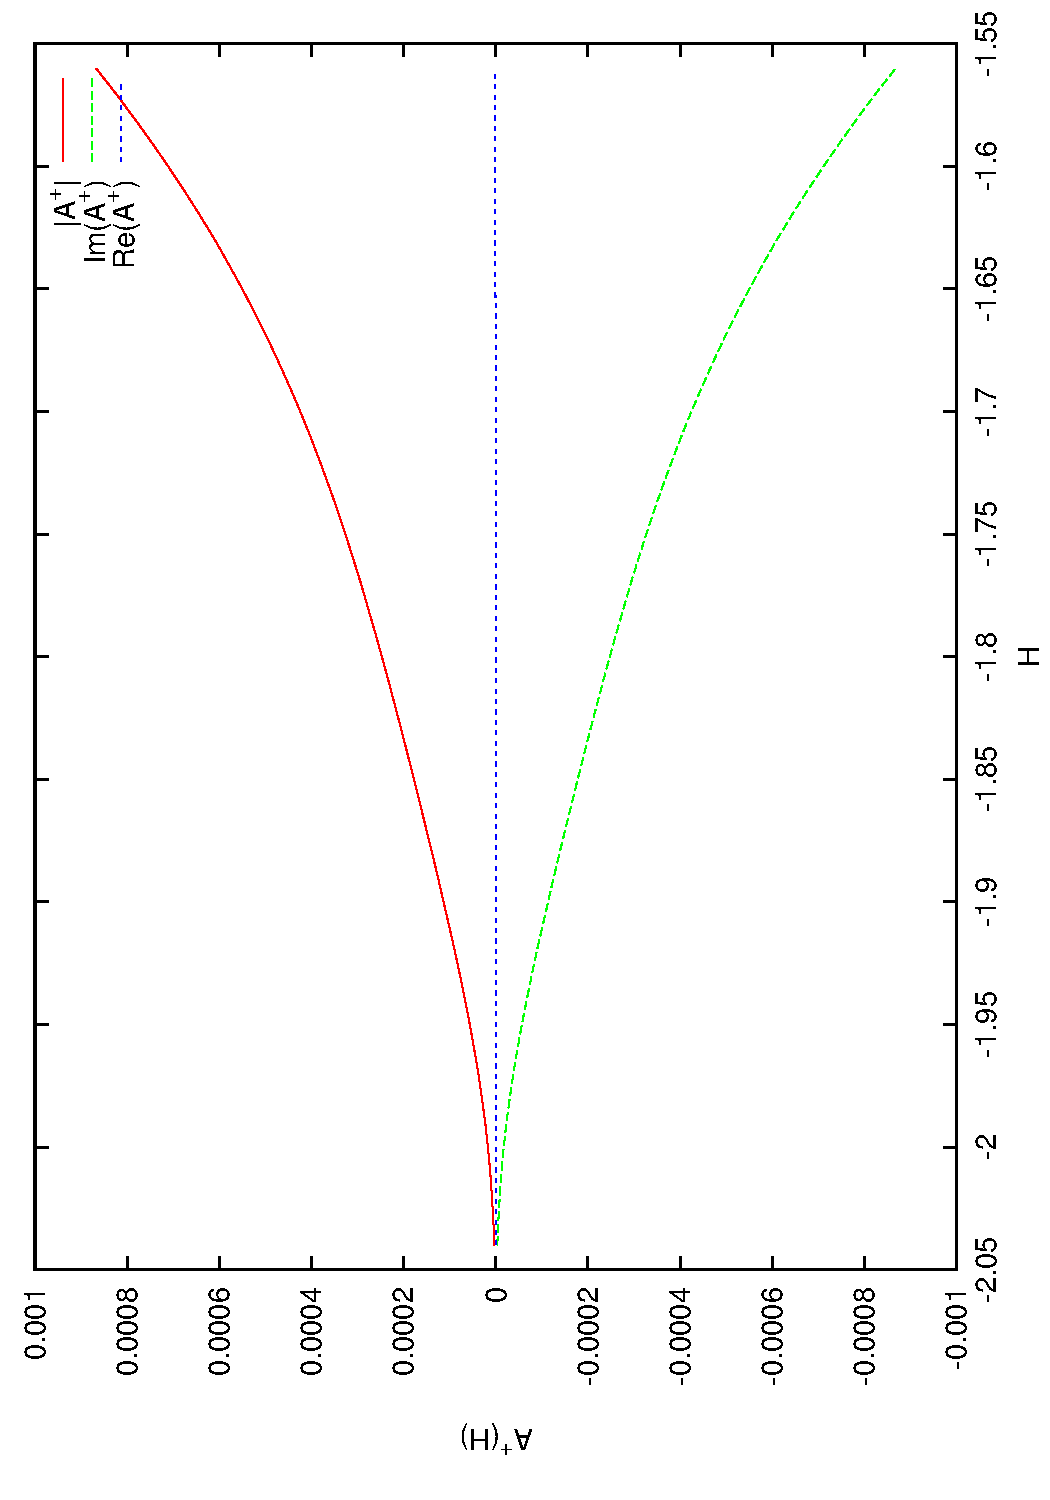
\includegraphics[angle=-90,width=\textwidth]{figs/inner_ell}
\caption{The complex integral $A^+$, as a function of energy level
$H$.}
\label{fig:inner_ell}
\end{figure}

Figure~\ref{fig:inner_ell} shows the complex integral $A^+$. We plot
its real part, imaginary part, and its modulus, as a function of
energy level $H$.

\subsection{Outer dynamics}

We need to compute the complex integral $\Omega^+(I)$ in Marcel's notes
\[ \Omega^+(I) = -B^+(I) - C^+(I), \]
where 
\[ B^+(I) = -\mu \int_0^{14M\pi} 
   f(\Phi_s(x_h))) e^{it(s)} - f(\Phi_s(x_p)) e^{i(t(s)+\omega_0^+)} ds, \]
\[ C^+(I) = -\mu \int_{-14M\pi}^0
   f(\Phi_s(x_h)) e^{it(s)} - f(\Phi_s(x_p) e^{i(t(s)-\omega_0^-)} ds. \]
where $\Phi_s$ denotes the flow of the reduced system, and
$x_h$, $x_p$ are the homoclinic and periodic points in the $g=0$ section.

\begin{figure}
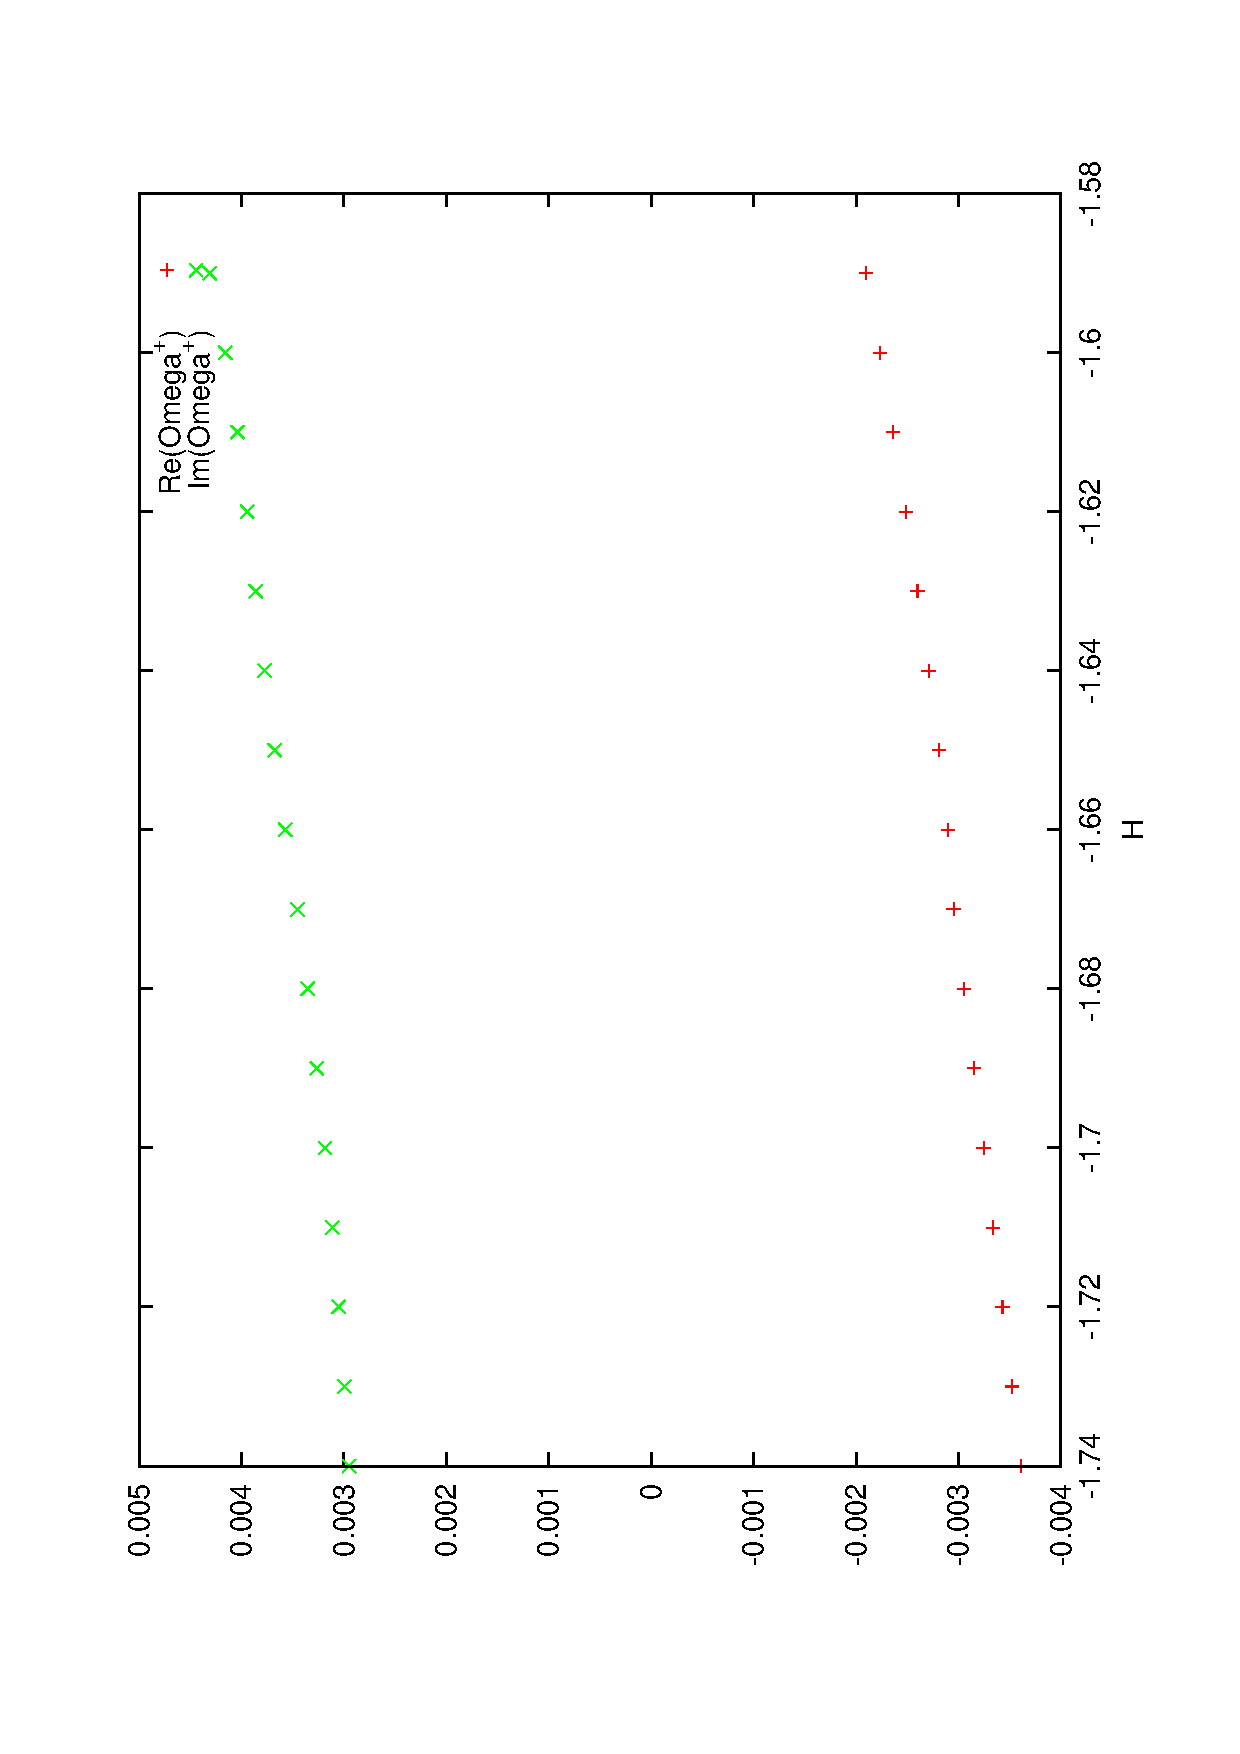
\includegraphics[angle=-90,width=\textwidth]{figs/Omega}
\caption{The complex integral $\Omega^+$, as a function of energy level
$H$.}
\label{fig:Omega}
\end{figure}

Figure~\ref{fig:Omega} shows the complex integral $\Omega^+$. We plot
its real part and imaginary part as a function of energy level $H$.

\section{Absence of common invariant curves}

To see that there are no common invariant curves it is enough to check
that the function
// \[ \tilde \Omega^+(I) = \Omega^+ - \frac{e^{i\omega_0}-1}{e^{iT_0}-1} A_1^+ \]
is non-zero for a range of energies, where
\begin{itemize}
\item $T_0$ is related to the inner map of the circular problem, and is
computed in program "periods".

\item $\omega_0$ is related to the outer map of the circular problem, and is
computed in program "omega".

\item $A_1^+$ is related to the inner map of the elliptic problem, and is
computed in program "inner\_ell".

\item $\Omega^+$ is related to the outer map of the elliptic problem, and is
computed in program "outer\_ell".
\end{itemize}

\begin{figure}
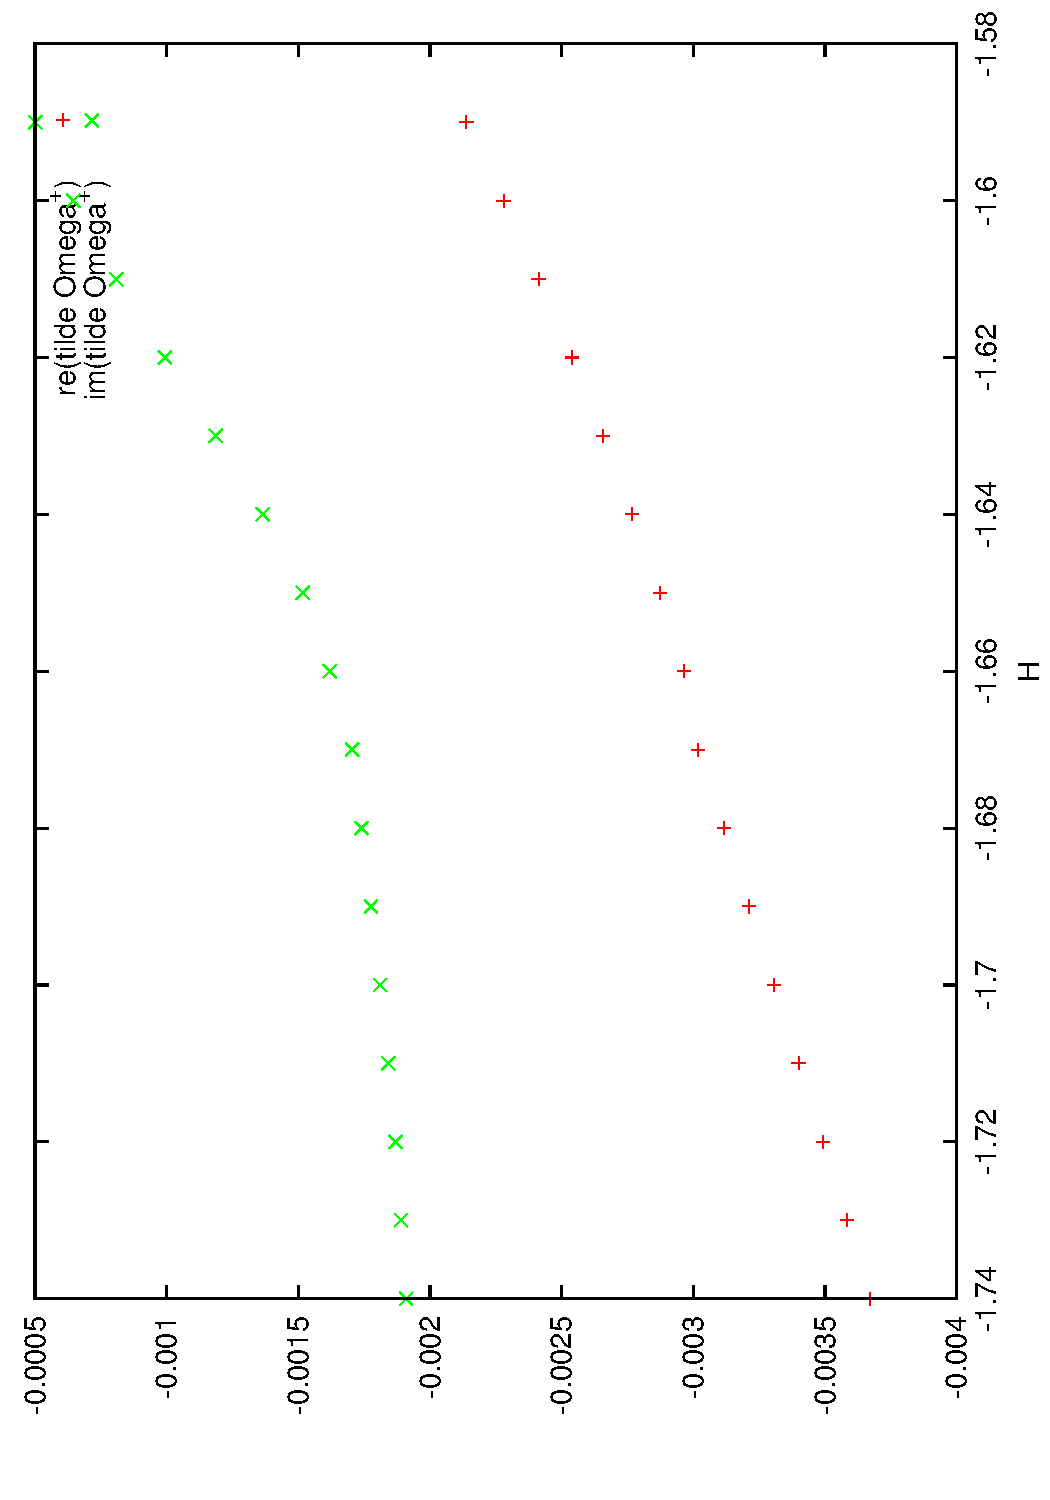
\includegraphics[angle=-90,width=\textwidth]{figs/tOmega}
\caption{The complex integral $\tilde \Omega^+$, as a function of energy level
$H$.}
\label{fig:tOmega}
\end{figure}

Figure~\ref{fig:tOmega} shows the complex integral $\tilde \Omega^+$. We plot
its real part and imaginary part as a function of energy level $H$.
Therefore, we see that indeed there are no common invariant curves.

\begin{comment}
\section{Variation of action $J$ in outer dynamics}

We would like to investigate the variation of the Jacobi constant $J$
along homoclinic tranjectories in the elliptic RTBP. 
We follow the notes be Jacques and Marcel in file e0.pdf.

Throughout this section, we will consider the circular RTBP in
rotating euclidean coordinates
\begin{subequations} \label{eq:RTBP_euclidean}
\begin{align}
H(x,y,p_x,p_y) &= \frac{1}{2}(p_x^2+p_y^2)+yp_x-xp_y-F(x,y)
\label{eq:RTBP_Hamiltonian} \\
F(x,y) &= \frac{1-\mu}{r_1}+\frac{\mu}{r_2} \\
r_1 &= ((x-\mu)^2+y^2)^{1/2} \\
r_2 &= ((x+(1-\mu))^2+y^2)^{1/2}
\end{align}
\end{subequations}
or in rotating polar coordinates
\begin{subequations} \label{eq:RTBP_polar}
\begin{align}
H_{polar}(r,\phi,R,G) &= \frac{1}{2}(R^2+\frac{G^2}{r^2})-G-F(r,\phi)
\\
F(r,\phi) &= \frac{1-\mu}{r_1}+\frac{\mu}{r_2} \\
r_1 &= r^2 + \mu^2 - 2\mu r\cos \phi \\
r_2 &= r^2 + (1-\mu)^2 + 2(1-\mu)r\cos \phi.
\end{align}
\end{subequations}

Let $\gamma(t)$ be a homoclinic trajectory of the circular RTBP like
the one found in the previous section.

Let $H_{ell}$ be the hamiltonian of the elliptic problem
\[ H_{ell} = J + e_0\Delta H_{ell}. \]

The variation of $J$ along $\gamma(t)$ is given to first order in the
eccentricity $e_0$ by the Melnikov integral
\begin{equation}\label{eq:Melnikov} 
\int_{-T}^{T'} \{ J, \Delta H_{ell} |_{e_0=0} \} \circ \gamma(t) dt,
\end{equation}
where the Jacobi constant $J$ coincides with the Hamiltonian,
$\Delta H_{ell} |_{e_0=0}$ is given in polar coordinates by
\begin{subequations}
\begin{align*} 
\Delta H_{ell} |_{e_0=0} &= -\frac{1-\mu}{\mu}
B(-r/\mu)-\frac{\mu}{1-\mu}B(r/(1-\mu)) \\
B(r) &= \frac{1}{2\Delta(r)^3}(2\cos t-3r\cos(\phi+t)+r\cos(\phi-t))
\\
\Delta(r) &= (r^2+1-2r\cos \phi)^{1/2},
\end{align*}
\end{subequations}
and the brackets denote Poisson brackets.

The limits of integration $-T,T$ should be taken large enough,
although the integral does not decay exponentially as $T,T'\to
\infty$. 
We will probably have to study the behaviour of the integral as a
function of $T,T'$.

Notice that in the previous section we have computed the homoclinic
trajectory in euclidean coordinates.
Thus we decide to tranform $\Delta H_{ell} |_{e_0=0}$ to euclidean
coordinates too, in order to compute integral~\eqref{eq:Melnikov}.

Recall that the transformation between euclidean coordinates
$x,y,p_x,p_y$ and polar coordinates $r,\phi,R,G$ is given by (cfr.
Szebehelly, section 7.5)
\begin{align*}
x &= r \cos \phi \\
y &= r \sin \phi \\
p_x &= R\cos \phi - \frac{G}{r}\sin \phi \\
p_y &= R\sin \phi + \frac{G}{r}\cos \phi
\end{align*}
and
\begin{align*}
r &= \sqrt{x^2+y^2} \\
\phi &= atan2(y,x) \\
R &= p_x\cos \phi + p_y\sin \phi \\
G &= r(-p_x\sin \phi + p_y\cos \phi).
\end{align*}

Applying this changes of coordinates to the expression of $\Delta
H_{ell}$, we obtain
\begin{subequations}
\begin{align}
\Delta(r)^2 &= x^2+y^2+1-2x \\
B(r) &= \frac{1}{2(x^2+y^2+1-2x)^{3/2}} (2\cos(t)-2x\cos(t)+4y\sin(t)) \\
B_1 := B(\frac{-r}{\mu}) &=
\frac{1}{2(\frac{x^2+y^2}{\mu^2}+1+\frac{2}{\mu}x)^{3/2}}
(2\cos(t)+\frac{2}{\mu}x\cos(t)-\frac{4}{\mu}y\sin(t)) \\
B_2 := B(\frac{r}{1-\mu}) &=
\frac{1}{2(\frac{x^2+y^2}{(1-\mu)^2}+1-\frac{2}{1-\mu}x)^{3/2}}
(2\cos(t)-\frac{2}{1-\mu}x\cos(t)+\frac{4}{1-\mu}y\sin(t)) \\
\Delta H_{ell} &= -\frac{1-\mu}{\mu} B_1(x,y,t;\mu) - \frac{\mu}{1-\mu}
B_2(x,y,t;\mu). \label{eq:DeltaH_ell}
\end{align}
\end{subequations}

Thus we have 
\begin{align*} 
\left\{J,\Delta H_{ell}\right\} = \left\{H,\Delta H_{ell}\right\} 
= \frac{\partial H}{\partial x} \frac{\partial\Delta H}{\partial p_x}
- \frac{\partial H}{\partial p_x} \frac{\partial\Delta H}{\partial x}
+ \frac{\partial H}{\partial y} \frac{\partial\Delta H}{\partial p_y}
- \frac{\partial H}{\partial p_y} \frac{\partial\Delta H}{\partial y}.
\end{align*}
Notice that the function $\Delta H_{ell}$ does not depend on
$p_x,p_y$. Hence the Poisson bracket reduces to
\begin{align*} 
\left\{H,\Delta H_{ell}\right\} = 
- \frac{\partial H}{\partial p_x} \frac{\partial\Delta H}{\partial x}
- \frac{\partial H}{\partial p_y} \frac{\partial\Delta H}{\partial y},
\end{align*}
with $H$ given by equation~\eqref{eq:RTBP_Hamiltonian} and $\Delta
H_{ell}$ given by equation~\eqref{eq:DeltaH_ell}.

We will start by considering a homoclinic orbit $\gamma$ that is
composed of $n=10$ forward iterates of the homoclinic point $z$ by
the Poincare map, and $m=10$ backward iterates.
We need to compute the integration time for this homoclinic.

\begin{verbatim}
roldan@pollo:~/research/splitting/homoclinic$ prtbp_2d <z_prtbp_2d.dat
#output: (x',p_x') integration_time
1.302614818060074e+00 -8.516834536255107e-03 4.418461961631185e+02
roldan@pollo:~/research/splitting/homoclinic$ prtbp_2d_inv
<z_prtbp_2d.dat
#output: (x',p_x') integration_time
1.302589128741115e+00 -7.470504613064666e-03 -4.378351198606701e+02
\end{verbatim}
Thus the backward integration time is $t_u=-4.378351198606701e+02$,
and the forward integration time is $t_s=4.418461961631185e+02$.

We also need to use the energy condition to derive the momentum $p_y$
of the homoclinic point from the fixed energy level $H$.

\begin{verbatim}
roldan@pollo:~/research/splitting/homoclinic$ hinv <hinv_z.dat
4.886772413841963e-01                             #output: p_y
\end{verbatim}
Thus $z=(2.998991488521247e+00, 0.0, -3.984065185921605e-01,
4.886772413841963e-01)$.

Before computing the Melnikov integral~\eqref{eq:Melnikov}, we
investigate the behavior of the integrand
\begin{equation} \label{eq:integrand}
f(t) = \{ J, \Delta H_{ell} |_{e_0=0} \} \circ \gamma(t).
\end{equation}
We compute the graph of the integrand $f(t)$ for an equispaced
sequence of points $t\in [-t_u,t_s]$:

\begin{verbatim}
roldan@pollo:~/research/splitting/integrand$ ./integrand >integrand.res
0.95387536e-3         # input: mu
# input: z=(x,y,p_x,p_y)
2.998991488521247e+00 0.0 -3.984065185921605e-01 4.886772413841963e-01
4.378351198606701e+02 4.418461961631185e+02    # input: t_u, t_s
\end{verbatim}

The integrand $f(t)$ is plotted in figure~\ref{fig:integrand}. 
As expected, the function $f(t)$ oscillates around zero.
Peaks roughly correspond to points in the discrete homoclinic orbit of
figure~\ref{fig:homoclinic}.

\begin{figure}
\subincludefrom{figs/}{integrand}
\caption{Integrand of Melnikov function.}
\label{fig:integrand}
\end{figure}

A closeup near $t=0$ shows several oscillations whose period is close
to $T=14\pi=43.982\dots$, see figure~\ref{fig:integrand_zoom}.

\begin{figure}
\subincludefrom{figs/}{integrand_zoom}
\caption{Closeup of integrand function $f(t)$.}
\label{fig:integrand_zoom}
\end{figure}

Finally, we compute the Melnikov integral~\eqref{eq:Melnikov} for our
homoclinic orbit, and integration limits $-T=-t_u$ and $T'=t_s$. We
use a standard numerical integrator from the GNU Scientific Library.
We ask for a relative error of $10^{-3}$ in the computation of the
integral.

\begin{verbatim}
roldan@pollo:~/research/splitting/melnikov$ ./melnikov
0.95387536e-3   # input: mu
# input: z=(x,y,px,py)
2.998991488521247e+00 0.0 -3.984065185921605e-01 4.886772413841963e-01
# input: t_u, t_s
-4.378351198606701e+02 4.418461961631185e+02
estimated error =  1.757e-03
estimated error =  1.256e-03
...
estimated error =  1.184e-03
estimated error =  4.085e-18
# output: Value of the Melnikov integral I
-2.587208996494296e-01
\end{verbatim}

\begin{rem}
Numerical remark.
We split the integral in several parts of size $t=7*(2\pi)$ in order
to compute it accurately.  This is motivated by the previous analysis
of the integrand (see figure~\ref{fig:integrand}).
\end{rem}

Let $t_0$ be the initial time, which determines the initial angle of
the rotating frame of coordinates.
Up to now, we have implicitly been using $t_0=0$, i.e. the primaries
are initially aligned with the horizontal axis (of the fixed frame).

The Melnikov integral actually depends on the value of $t_0$, because
the Hamiltonian $H_{ell}$ of the elliptic problem does depend on it:
\begin{equation}
M(\gamma,t_0):=\int_{-T}^{T'} \{ J, \Delta H_{ell} |_{e_0=0} \} \circ
(\gamma(s),t_0) ds.
\end{equation}
Figure~\ref{fig:timeshifts} shows how the value of the Melnikov
integral changes as we change the initial time $t_0$.

\begin{figure}
\subincludefrom{figs/}{timeshifts}
\caption{}
\label{fig:timeshifts}
\end{figure}

We would like to analyze the behavior of the Melnikov integral when $T\to \infty$.
When $t\to \infty$, the homoclinic approaches the periodic orbit,
except for a possible time shift $t_0$.
Thus we investigate the Melnikov integral on the unperturbed periodic
orbit $p(t)$ instead of the unperturbed homoclinic $\gamma(t)$.
Again, we do this for different values of the initial time $t_0$.
The result is shown in figure~\ref{fig:timeshiftspo}.

Remember that the periodic orbit for the circular RTBP becomes a
quasi-periodic orbit for the elliptic RTBP, since there is a slow
drift in the argument of the perihelion measured every $t=T_p$. 
This corresponds to slowly changing $t_0$. 

The $t_0$ time shift in our periodic orbit is exactly $\Delta
t_0:=T_p-7 T_J = T_p- 14\pi = 0.00285$. 
For a complete turn of the rotating frame, time must have shifted by
$2\pi$.
Thus the slow variable $t_0$ makes a full turn after $2\pi/\Delta t_0
= 2202.14$ turns of the asteroid along the periodic orbit (fast
variable).

Hence, acording to figure~\ref{fig:timeshiftspo}, the Melnikov
integral over the quasi-periodic orbit decreases for a very long time,
and then it increases for a very long time.

\begin{figure}
\subincludefrom{figs/}{timeshiftspo}
\caption{}
\label{fig:timeshiftspo}
\end{figure}

\end{comment}

\section{Connecting resonant 7:1 and 8:1 orbits}

Following Vadim's suggestion, we check to see if there is heteroclinic
connection between the periodic orbit $\Gamma_{7:1}$ with period
$T_{7:1}\approx 14\pi$, and the periodic orbit $\Gamma_{8:1}$ with period
$T_{8:1}\approx 16\pi$.

As before, we will compute the periodic orbits, their hyperbolic
invariant manifolds, and check if they intersect.

We look for these two periodic orbits in the same level of energy
$H=-1.6$. 
Notice that in section~\ref{sec:periodic_orbit} we used a slightly
different value $H=H_0$ (see equation~\eqref{eq:energy}).

We start by obtainig an approximation to the periodic orbits from the
2BP. I have written a simple script that, given a resonance, returns the
initial condition at the perihelion corresponding to that resonant periodic
orbit in the 2BP.

\begin{verbatim}
roldan@pollo:~/research/splitting$ bc -l initcond.bc 
Resonance (p/q, p=period of Asteroid, q=period of Jupiter)? 7/1
G = 1.46336205837340077849      # output: angular momentum
e = .64404909086496709969       # output: eccentricity
Initial condition at perihelion (in euclidean coords):
x = 1.30253319428569378555      # output: x
v_y = 1.12347390822228156181    # output: v_y

roldan@pollo:~/research/splitting$ bc -l initcond.bc 
Resonance (p/q, p=period of Asteroid, q=period of Jupiter)? 8/1
G = 1.47500000000000000000
e = .67534713296200495530
Initial condition at perihelion (in euclidean coords):
x = 1.29861146815198017877
v_y = 1.13582856472000335952
\end{verbatim}

Thus from the 2BP we have the following approximation to an initial
condition (at the perihelion):
\begin{align} 
(x,y,p_x,p_y)=(1.3025,0,0,1.1234) &\qquad \textrm{for }\Gamma_7 \\
(x,y,p_x,p_y)=(1.2986,0,0,1.1358) &\qquad \textrm{for }\Gamma_8. 
%(x,y,p_x,p_y)=(1.3003,0,0,1.1300) &\qquad \textrm{for }\Gamma_{15:2}.
\end{align}

%We start by checking these initial conditions give rise to approximate periodic
%orbits, integrating the corresponding solutions for one period of time.

%\begin{verbatim}
%roldan@pollo:~/research/splitting/connect78$ trtbp <trtbp_approx_po75.dat >per75.res 
%\end{verbatim}

We refine to obtain the true periodic orbits:

\begin{verbatim}
# Symmetric resonant 7:1 periodic orbit:
roldan@pollo:~/research/splitting/connect78$ portbpsym <portbpsym7.dat
iter =   1 x =  1.3019610882, PX =  1.0037e-05
iter =   2 x =  1.3019618967, PX =  2.1996e-11
iter =   3 x =  1.3019618967, PX =  1.9761e-15
# output: x, period/2
1.301961896721998e+00 2.199257575905967e+01

# Symmetric resonant 8:1 periodic orbit:
roldan@pollo:~/research/splitting/connect78$ portbpsym <portbpsym8.dat
iter =   1 x =  1.2980565203, PX = -4.6678e-06
iter =   2 x =  1.2980568305, PX = -1.9871e-12
iter =   3 x =  1.2980568305, PX =  6.4560e-16
# output: x, period/2
1.298056830506968e+00 2.513409782621527e+01
\end{verbatim}
Thus we find symmetric periodic orbits passing through the points
$(x,p_x)=(1.30196,0)$ and $(x,p_x)=(1.29805,0)$, with the correct periods
$T_{7:1}\simeq14\pi$ and $T_{8:1}\simeq16\pi$.

% ********************** BEGIN COMMENT ********************
\begin{comment}
We derive the value of $p_y$ from the energy condition:
\begin{verbatim}
# Resonant 7:1 periodic orbit:
roldan@pollo:~/research/splitting/connect78$ hinv
0.95387536e-3 -1.6                      # input: mu H
1.301961896721998e+00 0 0               # input: x y p_x
1.12347390822228156181                  # input: p_y estimate (2BP)
1.123812946399732e+00                   # output: p_y

# Resonant 8:1 periodic orbit:
roldan@pollo:~/research/splitting/connect78$ hinv
0.95387536e-3 -1.6
1.298056830506968e+00 0 0
1.13582856472000335952
1.136165165357439e+00
\end{verbatim}

Finally, we compute the periodic orbits:
\begin{verbatim}
roldan@pollo:~/research/splitting/connect78$ trtbp <trtbp7.dat >trtbp7.res
\end{verbatim}

The periodic orbits $\Gamma_{7:1}$ and $\Gamma_{8:1}$ are
plotted in figures~\ref{fig:approx_per78_rot}
and~\ref{fig:approx_per78_nonrot}.

\begin{figure}
\subincludefrom{figs/}{approx_per78_rot}
\caption{}
\label{fig:approx_per78_rot}
\end{figure}

\begin{figure}
\subincludefrom{figs/}{approx_per78_nonrot}
\caption{}
\label{fig:approx_per78_nonrot}
\end{figure}
\end{comment}
% ********************** END COMMENT ********************

After computing the periodic orbits, we compute their hyperbolic
invariant manifolds.
We compute the derivative of the 2D Poincare map evaluated at the
fixed point:

\begin{verbatim}
# Resonant 7:1 periodic orbit:
roldan@pollo:~/research/splitting/connect78$ dprtbp_2d <dprtbp_2d_7.dat 
 1.2658907713e+00  1.6232238702e-04
 3.7116225998e+03  1.2658907674e+00

# Resonant 8:1 periodic orbit:
roldan@pollo:~/research/splitting/connect78$ dprtbp_2d <dprtbp_2d_8.dat 
 1.3342774290e+00  1.2561294528e-04
 6.2119095309e+03  1.3342774247e+00
\end{verbatim}

Compute eigenvalues/vectors:

\begin{verbatim}
# Resonant 7:1 periodic orbit:
octave:1> M=[
> 1.2658907713e+00,  1.6232238702e-04;
> 3.7116225998e+03,  1.2658907674e+00 ];
octave:2> [evects, evals] = eig(M);
octave:3> format long
octave:4> diag(evals)
ans =

  2.042086260265088
  0.489695278434912

octave:5> evects
evects =

    2.09125646539071e-04   -2.09125645488317e-04
    9.99999978133232e-01    9.99999978133232e-01

octave:6> # Test symplecticity:
octave:6> 2.042086260265088*0.489695278434912
ans = 0.999999999808620

# Resonant 8:1 periodic orbit:
octave:7> M=[
>  1.3342774290e+00,  1.2561294528e-04;
>  6.2119095309e+03,  1.3342774247e+00];
octave:8> [evects, evals] = eig(M);
octave:9> diag(evals)
ans =

  2.217621217222272
  0.450933636477728

octave:10> evects
evects =

    1.42201649782093e-04   -1.42201649089874e-04
    9.99999989889345e-01    9.99999989889345e-01

octave:11> # Test symplecticity:
octave:11> 2.217621217222272*0.450933636477728
ans = 0.999999999812205
\end{verbatim}

Thus $\Gamma_{8}$ is slightly more hyperbolic than $\Gamma_{7}$.

Finally, compute the invariant manifolds:
\begin{verbatim}
roldan@pollo:~/research/splitting/connect78$ invmfld <stmfld7.dat
>stmfld7.res 
Estimated error of manifold: 4.888741e-09

roldan@pollo:~/research/splitting/connect78$ invmfld <unstmfld8.dat
>unstmfld8.res 
Estimated error of manifold: 7.755391e-09
\end{verbatim}
The manifolds are plotted in figures~\ref{fig:invmfld78}
and~\ref{fig:invmfld78_zoom}. 

\begin{figure}
\subincludefrom{figs/}{invmfld78}
\caption{}
\label{fig:invmfld78}
\end{figure}

\begin{figure}
\subincludefrom{figs/}{invmfld78_zoom}
\caption{}
\label{fig:invmfld78_zoom}
\end{figure}

Unfortunately, the pieces of manifolds that we have computed so far do
not intersect. 

\section{Connecting resonant 22:3 and 23:3 orbits}

Let's try other resonances in between the 7:1 and the
8:1.
We start with e.g. the 15:2. The associated periodic orbit should be closer,
and the manifolds are more likely to intersect.

\begin{verbatim}
# 15:2 resonant periodic orbit
roldan@pollo:~/research/splitting$ bc -l initcond.bc 
Resonance (p/q, p=period of Asteroid, q=period of Jupiter)? 7.5
G = 1.46950441196103788015
e = .66060909407979723042
Initial condition at perihelion (in euclidean coords):
x = 1.30039226237622183524
v_y = 1.13004702848338658691

roldan@pollo:~/research/splitting/connect78$ portbpsym <portbpsym152.dat
iter =   1 x =  1.2899133592, PX =  4.3411e-02
iter =   2 x =  1.2885270066, PX =  9.1810e-04
iter =   3 x =  1.2884965118, PX =  2.8660e-07
iter =   4 x =  1.2884965023, PX =  2.5271e-14
# output: x, half_period
1.288496502319741e+00 4.398345642247595e+01
\end{verbatim}
The problem when trying to compute the 15:2 periodic orbit is that the
Newton method converges to the wrong periodic orbit. In particular,
note that the half period obtained is $43.983$, whereas we are looking for
half-period $15\pi=47.123$.

Let's try now the 22:3 and 23:3 periodic orbits.
Initial conditions:
\begin{verbatim}
# 22:3 resonant periodic orbit
Resonance (p/q, p=period of Asteroid, q=period of Jupiter)? 7.33333333333333333333
G = 1.46\ 753462083519417937
e = .65530892644628352172
Initial condition at perihelion (in euclidean coords):
x = 1.30106098562127554633
v_y = 1.12795221519491267400

# 23:3 resonant periodic orbit
Resonance (p/q, p=period of Asteroid, q=period of Jupiter)? 7.66666666666666666666
G = 1.47\ 140257174563659372
e = .66570757089910450874
Initial condition at perihelion (in euclidean coords):
x = 1.29976327535754083319
v_y = 1.13205427453001467915
\end{verbatim}

Refine periodic orbits:
\begin{verbatim}
# 22:3 resonant periodic orbit
roldan@pollo:~/research/splitting/connect78$ portbpsym <portbpsym223.dat 
iter =   1 x =  1.3005396932, PX =  4.2305e-03
iter =   2 x =  1.3002987781, PX =  2.0885e-03
iter =   3 x =  1.3013461566, PX =  3.0274e-02
...
iter =  10 x =  1.2999256706, PX = -3.0029e-09
main: unable to find periodic orbit up to desired accuracy
1.299925670618873e+00 6.914163447968416e+01

# 23:3 resonant periodic orbit
roldan@pollo:~/research/splitting/connect78$ portbpsym <portbpsym233.dat 
iter =   1 x =  1.2997530192, PX = -1.8363e-04
iter =   2 x =  1.2997521734, PX = -1.2262e-06
iter =   3 x =  1.2997521677, PX = -5.6028e-11
iter =   4 x =  1.2997521677, PX = -3.4963e-15
1.299752167708986e+00 7.228528203030096e+01
\end{verbatim}
This time, the half-periods are correct. We are not able to obtain the
22:3 with a lot of accuracy, only $10^{-9}$, but we will use this
orbit nonetheless.

Derivative (2D):
\begin{verbatim}
roldan@pollo:~/research/splitting/connect78$ dprtbp_2d <dprtbp_2d_223.dat 
 1.1410166321e+02  2.8682531086e-02
 5.0220818044e+05  1.2625233809e+02

roldan@pollo:~/research/splitting/connect78$ dprtbp_2d <dprtbp_2d_233.dat 
 2.7683523791e+02  6.9331197838e-02
 1.1053772888e+06  2.7683661967e+02
\end{verbatim}

Eigenvalues/vectors:
\begin{verbatim}
# Resonant 22:3 periodic orbit:
octave:1> M=[
> 1.1410166321e+02,  2.8682531086e-02;
> 5.0220818044e+05,  1.2625233809e+02];
octave:2> [evects, evals] = eig(M);
octave:3> format long
octave:4> diag(evals)
ans =

   4.16065641549206e-03
   2.40349840643585e+02

octave:5> evects
evects =

   -2.51386134996544e-04   -2.27191638951380e-04
    9.99999968402505e-01   -9.99999974191979e-01

octave:6> # Test symplecticity:
octave:6> 4.16065641549206e-03*2.40349840643585e+02
ans = 1.00001310643623

# Resonant 23:3 periodic orbit:
octave:7> M=[2.7683523791e+02,  6.9331197838e-02;
> 1.1053772888e+06,  2.7683661967e+02];
octave:8> [evects, evals] = eig(M);
octave:9> diag(evals)
ans =

   1.80608128806509e-03
   5.53670051498712e+02

octave:10> evects
evects =

   -2.50443724248595e-04   -2.50442474213983e-04
    9.99999968638970e-01   -9.99999968639283e-01

octave:11> # Test symplecticity:
octave:11> 1.80608128806509e-03*5.53670051498712e+02
ans = 0.999973119773858
\end{verbatim}

\end{document}
